%%%%%%%%%%%%%%%%%%%%%%%%%%%%%%%%%%%%%%%%%%
%%% NORMALMENTE NO ES NECESARIO HACER 
%%% CAMBIOS EN ESTA PARTE DEL DOCUMENTO
%%%%%%%%%%%%%%%%%%%%%%%%%%%%%%%%%%%%%%%%%%


%:Clase del documento
\documentclass[fontsize=11pt, Myfinal=true, twoside, numbers=noenddot]{scrbook}
%Minion=true, English=true, Myfinal=true

%:Paquete de estilos propuesto
\usepackage{libroETSI}

%:Paquete específico para cargar tikz (y sus librerías) y pgfplots
\usepackage{dtsc-creafig}

%:Paquete para notaciones específicas
\usepackage{notacion}

%:Paquete para incorporar aspectos concretos de la edición
\usepackage{edicionPFC}

% Paquete para incluir epígrafes en los capítulos
\usepackage{epigraph}


%:Para modificar fácilmente la fuente del texto.
\makeatletter
\ifdtsc@Minion % Queremos utilizar la fuente Minion y lo hemos declarado al principio
	\ifluatex
		\setmainfont[Renderer=Basic, Ligatures=TeX,	% Fuente del texto 
		Scale=1.01,
		]{Minion Pro}
   		% En este caso conviene modificar ligeramente el tamaño de las fuentes matemáticas
		\DeclareMathSizes{10}{10.5}{7.35}{5.25}
		\DeclareMathSizes{10.95}{11.55}{8.08}{5.77}
		\DeclareMathSizes{12}{12.6}{8.82}{6.3}
%		\setmainfont[Renderer=Basic, Ligatures=TeX,	% Fuente del texto 
%		]{Adobe Garamond Pro}
%		\setmainfont[Renderer=Basic, Ligatures=TeX,	% Fuente del texto 
%		]{Palatino LT Std}
	\fi
\else
	\ifluatex
		% Para utilizar la fuente Times New Roman, o alguna otra que se tenga instalada
		\setmainfont[Renderer=Basic, Ligatures=TeX,	% Fuente del texto 
		Scale=1.0,
		]{Times New Roman}
	\else
		\usepackage{tgtermes} 	%clone of Times
		%\usepackage[default]{droidserif}
		%\usepackage{anttor} 	
	\fi
\fi
\makeatother

% Formato A4
\geometry
{paperheight=297mm,%
paperwidth=210mm,%
top=25mm,%
headsep=8.5mm,%
includefoot, 
textheight=240mm, 
textwidth=150mm, 
bindingoffset=0mm, 
twoside}

\usepackage[a4,center]{crop}%para poner las cruces de esquina de página, poner la opción cross

%:Esquema de numeración por defecto
\setenumerate[1]{label=\normalfont\bfseries{\arabic*.}, leftmargin=*, labelindent=\parindent}
\setenumerate[2]{label=\normalfont\bfseries{\alph*}), leftmargin=*}
\setenumerate[3]{label=\normalfont\bfseries{\roman*.}, leftmargin=*}
\setlist{itemsep=.1em}
\setlength{\parindent}{1.0 em}

\setcounter{tocdepth}{4}						% El nivel hasta el que se muestra el índice 


%%%%%%%%%%%%%%%%%%%%%%%%%%%%%%%%%%%%%%%%%%
%%% A PARTIR DE AQUÍ HAY QUE EDITAR
%%%%%%%%%%%%%%%%%%%%%%%%%%%%%%%%%%%%%%%%%%

% Ejemplo de Glosario
\newacronym[type=main]{ETSI}{ETSI}{Escuela Técnica Superior de Ingeniería}
\newacronym[type=main]{US}{US}{Universidad de Sevilla}
\newacronym[type=main]{DMC}{DMC}{Canal Discreto sin Memoria}


\makeindex
\makeglossaries %Si no se quiere el glosario, comentar esta línea.

\setlength{\parskip}{4pt}


%:Empieza el documento

\begin{document}

%PORTADA
%ver edicionPFC.sty para modificaciones

%:Para crear la portada y la portada interior (pagina titular)
\titulo{Integración de robot manipulador con \mbox{posicionador} basado en Arduino} %\mbox evita que se divida una palabra al cambiar de línea
\autor{Antonio Pérez García}
\director{Luis Fernando Castaño Castaño}
\titulodirector{Profesor Contratado Doctor}

\departamento{Dpto. Ingeniería de Sistemas y Automática}
\centro{Escuela Técnica Superior de Ingeniería}
\universidad{Universidad de Sevilla}
\titulacion{Grado en Ingeniería en Tecnologías Industriales}
\fecha{2022}
\nombretrabajo{Trabajo Fin de Grado} %Proyecto fin de Máster,....

\hypersetup
	{
 	linkcolor=black, %Tocar para poner color en enlaces
	pdfauthor={\elautor},
	pdftitle={\nombretrabajo,\eltitulo}, 
	pdfkeywords={Latex, edición, formato de texto}	
	 }

\portadaPFC{figuras/LogoUS.pdf}{figuras/LogoTSC.pdf} %logo de la Universidad y logo del departamento, si lo hubiera. Para cambiar el pie de página con los logos, debe editarse el fichero ediciónPFC.sty

%Fin Portada

%:Todo lo que constituye la primera parte del libro que no es el cuerpo del libro en realidad
\frontmatter
\pagenumbering{Roman} %Pone la numeración en mayúscula (En español parece que es obligatorio)

%\include{dedicatoria/dedicatoria}%¿Comentar para proyectos/tesis?
% !TEX root =../LibroTipoETSI.tex
\chapter*{Agradecimientos}
%\pagestyle{especial}
\pagestyle{empty}
%\chaptermark{Agradecimientos}
\phantomsection
%\addcontentsline{toc}{listasf}{Agradecimientos}
%\vspace{1cm}
%{\huge{Agradecimientos}}
%\vspace{1cm}

\lettrine[lraise=-0.1, lines=2, loversize=0.25]{E}{l} trabajo de fin de grado
es la culminación de mucho esfuerzo realizado durante años de mis padres Antonio
y Rosario. Agradezco su paciencia y apoyo durante todo este tiempo.

{\flushleft{\hfill \emph{Antonio Pérez García}}}%
\vspace{-.3cm}
%{\flushleft{\hfill \emph{Subdirección de Comunicaciones y Recursos Comunes}}}%
{\flushleft{\hfill \emph{Sevilla, 2022}}}%

%PFC/PFM/TESIS
% !TEX root =../main.tex
\chapter*{Resumen}
\pagestyle{especial}
\chaptermark{Resumen}
\phantomsection
\addcontentsline{toc}{listasf}{Resumen}

\lettrine[lraise=-0.1, lines=2, loversize=0.2]{E}n el laboratorio de Automática
de la Escuela Técnica Superior de Ingeniería de la Universidad de Sevilla 
hay robots de la marca ABB destinados a prácticas para alumnos. Durante estas 
prácticas es común la invasión del espacio de trabajo de los robots. El objetivo de
este proyecto es reducir 
la exposición a riesgos asociados a estos trabajos se introducen cintas transportadoras
que permiten el movimiento de piezas sin peligro para los alumnos. Para ello,
se desarrolla un dispositivo que permite el uso de dicha cinta de forma segura, 
además de dar información relevante sobre la posición de las piezas al robot.
El sistema está compuesto de un Arduino que posiciona las piezas en los ejes de la cinta
mediante un encoder y un calibre digital. También cuenta con una placa electrónica que
centraliza todas las conexiones y permite el funcionamiento para los distintos modos establecidos
según las necesidades de los alumnos.
Además, el sistema está pensado para ser fácilmente reparable, empleando piezas 
estandarizadas existentes en el mercado para sustituirlas en caso de ser necesario.
De esta forma se pone solución a un problema habitual de los laboratorios de prácticas con brazos
robóticos haciendo de este lugar un lugar más seguro para estudiantes y profesores.


\chapter*{Abstract}
\pagestyle{especial}
\chaptermark{Abstract}
\phantomsection
\addcontentsline{toc}{listasf}{Abstract}

\lettrine[lraise=-0.1, lines=2, loversize=0.2]{I}{n} the lab of automatics

% Índice abreviado 
% El índice abreviado se incluye también en algunos libros, con menor detalle que el completo. Descomentar las siguientes líneas.
\cleardoublepage
\phantomsection
\addcontentsline{toc}{listasf}{Índice Abreviado}
\pagestyle{especial}
\shorttoc{Índice Abreviado}{1}

%Índice normal, el completo
\cleardoublepage
\phantomsection
\pagestyle{especial}
\tableofcontents

\chapter*{\notationname}
\pagestyle{especial}
\chaptermark{\notationname}
\phantomsection
\addcontentsline{toc}{listasf}{\notationname}
%\section*{Notación}
%\begin{table}[htbp]
\begin{longtable}{p{3cm}p{8.5cm}}

%$\displaystyle D$ & Tasa de símbolos  (sim/s) \\
%$\displaystyle R_b$ & Tasa binaria (bit/s) \\
%$\displaystyle T$ & Tiempo de símbolo (s) \\
%$\displaystyle T_{b}$ & Tiempo de bit (s) \\
%$W\left( {t} \right)$ & Ruido blanco\\
%$w\left( {t} \right)$ & Función muestra de un ruido blanco\\
%$\displaystyle h_{c}\left( {t} \right)$ & Respuesta impulsiva de un canal LTI continuo en el tiempo\\
%$\displaystyle H_{c}\left( {\omega} \right)$ & Respuesta en frecuencia de un canal LTI continuo en el tiempo\\
%$\displaystyle h_{c}\left( {\tau;t} \right)$ & Respuesta impulsiva de un canal LTV continuo en el tiempo\\
%$\displaystyle H_{c}\left( {\omega;t} \right)$ & Respuesta en frecuencia de un canal LTV continuo en el tiempo\\
%$\displaystyle h_{c}\left( {n} \right)$ & Respuesta impulsiva de un canal LTI discreto en el tiempo\\
%$\displaystyle H_{c}\left( {\Omega} \right)$ & Respuesta en frecuencia de un canal LTI discreto en el tiempo\\
ABB & Cuerpo de los números reales \\
$\CC$ & Cuerpo de los números complejos\\
$\left\| \vc{v} \right\|$ & Norma del vector $\vc{v}$ \\
$\left\langle {\vc{v}, \vc{w}} \right\rangle$ & Producto escalar de los vectores $\vc{v}$ y $\vc{w}$\\
$\left| {\vc{A}} \right|$ &Determinante de la matriz cuadrada $\vc{A}$\\
$\textrm{det}\left( {\vc{A}} \right)$ &Determinante de la matriz (cuadrada) $\vc{A}$\\
$\vc{A}\trs$ & Transpuesto de $\vc{A}$\\
$\vc{A}\inv$ & Inversa de la matriz $\vc{A}$\\
$\vc{A}{\psd}$ & Matriz pseudoinversa de la matriz $\vc{A}$\\
$\vc{A}\her$ & Transpuesto  y conjugado de $\vc{A}$\\
$\vc{A}\cnj$ & Conjugado\\
c.t.p. & En casi todos los puntos\\
c.q.d. & Como queríamos demostrar\\
\ensuremath{\blacksquare}& Como queríamos demostrar\\
\ensuremath{\square}& Fin de la solución\\
e.o.c. & En cualquier otro caso\\
$\e$ & número e\\
$\xp{x}$ & Exponencial compleja\\
$\xppi{x}$ & Exponencial compleja con $2\pi$\\
$\nxp{x}$ & Exponencial compleja negativa\\
$\nxppi{x}$ & Exponencial compleja negativa con $2\pi$\\
$\re$ & Parte real\\
$\im$ & Parte imaginaria\\
$\sen$ & Función seno \\
$\tg$ & Función tangente \\
$\arctg$ & Función arco tangente \\
$\sento{y}{x}$ & Función seno de $x$  elevado a $y$\\
$\costo{y}{x}$ & Función coseno de $x$  elevado a $y$\\
$\sa$ & Función sampling \\
$\sgn$ & Función signo \\
$\rect$ & Función rectángulo \\
$\sinc$ & Función sinc\\
$\pder{y}{x} $ & Derivada parcial de $y$ respecto a $x$\\
$x\gra$ & Notación de grado, $x$ grados.\\
%
%$C_{XY}$& covarianza  de dos variables aleatorias reales $X$ e $Y$\\
%$R_{XY}$& correlación  de dos variables aleatorias reales $X$ e $Y$\\
%$\rho_{XY}$ &Coeficiente de correlación de las variables aleatorias reales $X$  e $Y$\\
%$\vc{Z}$ & Vector aleatorio complejo\\
%$\displaystyle F_{X}\left( {\cdot} \right)$ & Función de distribución de la variable aleatoria $X$ \\
%$\displaystyle f_{X}\left( {\cdot} \right)$ & Función densidad de probabilidad de la variable aleatoria $X$ \\
%$p_{X}\left( {\cdot} \right)$ & Función masa de probabilidad de la variable aleatoria discreta $X$ \\
%
$\Pr\left( {A} \right)$ & Probabilidad del suceso $A$ \\
$\displaystyle E\left[ {X} \right]$ & Valor esperado de la variable aleatoria $X$ \\
$\si{X}$ & Varianza de la variable aleatoria $X$\\
$\sim f_{X}\left( {x} \right)$ & Distribuido siguiendo la función densidad de probabilidad $f_{X}\left( {x} \right)$\\
%
$\gauss{m_{X}}{\si{X}}$ &Distribución gaussiana para la variable aleatoria X, de media $m_{X}$ y varianza $\si{X}$ \\
$\id{n}$ & Matriz identidad de dimensión $n$\\
$\diag{\vc{x}}$ & Matriz diagonal a partir del vector $\vc{x}$\\
$\diag{\vc{A}}$ & Vector diagonal de la matriz $\vc{A}$\\
$\snr$& Signal-to-noise ratio \\
$\mse$ & Minimum square error\\
$\talq$ & Tal que \\
$\eqdef$ & Igual por definición \\
$\norm{\vc{x}}$ & Norma-2 del vector $\vc{x}$\\
$\card{\vc{{A}}}$ & Cardinal, número de elementos del conjunto $\vc{A}$\\
$\xyz{\vc{x}}{i}{n}$ & Elementos $i$, de 1 a $n$, del vector $\vc{x}$\\
%\newcommand{\xyz}[3]{\ensuremath{#1_{#2},#2=1,2,\ldots,#3}}
$\df{x}$& Diferencial de $x$\\
$\le$ & Menor o igual \\
$\ge$ & Mayor o igual \\
$\BL$ & Backslash \\
$\iff$ & Si y sólo si \\
$x=a+3\eqexpl{a=1} 4 $& Igual con explicación \\
$\tfrac{a}{b}$ & Fracción con estilo pequeño, $a/b$ \\
$\inc$ & Incremento \\
$b\ten{a}$ & Formato científico \\
$\tendsub{x}$ & Tiende, con x \\
$\ord$ & Orden\\
$\tm$ & Trade Mark\\
$\E[x]$ & Esperanza matemática de x\\
$\covm{\vc{x}}$ & Matriz de covarianza de $\vc{x}$\\
$\corrm{\vc{x}}$ & Matriz de correlación de $\vc{x}$\\
$\si{x}$ & Varianza de x \\


\end{longtable}
\newpage
%\end{table}
%


%\phantomsection
%\addcontentsline{toc}{listasf}{Acrónimos}
%\section*{Acrónimos}
%\begin{table}[htbp]
%\begin{tabular}{p{2cm}p{10cm}}
%Escuela Técnica Superior de In
%LTI & Lineal Invariante con el Tiempo \\
%LTV& Lineal Variable con el Tiempo\\
%AWGN& Ruido blanco gaussiano aditivo\\
%DMS& Fuente discreta sin memoria\\
%AEP& Propiedad de equipartición asintótica\\
%WLLN& Ley Débil de los Grandes Números\\
%DMC& Canal Discreto sin Memoria\\
%BSC& Canal Simétrico Binario\\
%BEC& Canal Binario con Borrado\\
%\end{tabular}
%\end{table}


%\nota{El libro de Lapidoth tiene una excelente recopilación.} %No incluir si no se quiere, comentándolo

%:Empieza el contenido del libro
\mainmatter

%:Página por defecto
\pagestyle{esitscCD}

%:Los diferentes capítulos, en carpetas separadas
%

\chapter{Guía de Uso}\label{chp-01}


%\lettrine[lraise=0.7, lines=1, loversize=-0.25]{E}{n}
\lettrine[lraise=-0.1, lines=2, loversize=0.2]{E}{n} este capítulo vamos a describir las partes de las que consta un documento tipo, cómo deben interpretarse los diferentes comandos que se han definido para su confección, los \indexit{paquetes} (conjunto de sentencias de \LaTeX\ escritas y desarrolladas por diversos autores) que se han cargados y el porqué de los mismos, elecciones realizadas en cuanto a la edición, el porqué de determinadas fuentes, etc. 

Hay mucho de elección personal en lo que sigue y únicamente se justifica desde el gusto personal de quienes escribimos esto. No pretendemos por ello sentar precedentes, obligaciones ni restricciones a quien desee utilizar este documento. En cualquier caso, esperamos que su lectura sea provechosa para la confección y edición de libros, apuntes de clase, proyectos, etc.

\LaTeX se ha convertido de hecho en el procesador de texto estándar para la edición de documentos científicos. Este libro está escrito precisamente en \LaTeX, haciendo uso de la plantilla que hemos diseñado y al escribir un libro sobre cómo escribir un libro en \LaTeX\  y cómo hacer uso de esta plantilla, estamos entrando muchas veces en una redundancia evidente.

Estas páginas no constituyen un manual de \LaTeX,  ni lo pretendemos, ya que existen incontables y buenas referencias sobre este tema. El objetivo es describir los aspectos formales que deseamos se puedan incorporar a cualquier texto producido en la Escuela.  También, como la mayoría de nuestra producción científica utiliza ampliamente las fórmulas matemáticas, incluimos algunos consejos sobre la escritura de las mismas, para lo que hemos utilizado las notas preparadas en \cite{moser}. Asimismo resulta muy interesante el libro \cite{gratzer}.

Por último, puesto que los ficheros fuentes de este documento están disponibles, esperamos que los mismos faciliten la utilización de los distintos elementos de edición.

\section{Cómo usar los  estilos de documento de la ETSI}\label{sec-00}

Una de las bondades del \LaTeX\ es que una vez definido el estilo, formado por un conjunto de paquetes y adaptaciones de los mismos, la escritura de un texto se reduce a dominar una serie de comandos. En nuestro caso, se presenta este documento como ejemplo de uso de estos comandos. En este capítulo encontrará detalles técnicos sobre la estructura del documento y una breve introducción sobre algunos de los elementos del estilo diseñado, puesto que en el Capítulo \ref{chap:estilo} se estudian detalladamente todos sus componentes. También encontrará instrucciones de cómo compilar el documento. Para usar esta hoja de estilo, se recomienda leer el Capítulo \ref{chap:CAPEJ} y Capítulo \ref{chap:CAPPB} como ejemplos de capítulos donde se incluyen la mayoría de los comandos que pueden ser de utilidad en la redacción de un texto técnico. 

El archivo \ttcolor{libroTipoETSI.tex} es el archivo principal, que tiene una serie de comandos para incluir las distintas partes que se necesiten. Muchas de estas partes se han incluido separadamente en carpetas, por comodidad. Este archivo lo hemos modificado levemente para utilizarlo como formato para proyecto fin de carrera/grado/máster. El resultado se incluye en un fichero con nombre \ttcolor{pfcTipoETSI.tex}. Y también se incluye un formato para tesis \ttcolor{tesisTipoETSI.tex}

Los datos necesarios para generar la cubierta y demás hojas iniciales se incluyen al comienzo de estos ficheros: el título del proyecto, autores, el nombre del departamento, etc. Si necesita retocar la cubierta  (por ejemplo el ancho de la imagen utilizada)  tendrá que modificar directamente el fichero \ttcolor{edicionLibro.sty}, que es el fichero al que se llama para generarla. Si quiere, también, puede retocar la imagen de fondo. Todo esto se explica en un apartado más adelante. Para los restantes tipos de documentos, estas modificaciones hay que hacerlas en los ficheros \ttcolor{edicionPFC.tex} y \ttcolor{edicionTesis.sty}.

Así, para empezar a utilizar este documento, basta que empiece modificando los ficheros \ttcolor{libroTipoETSI.tex} (ó \ttcolor{pfcTipoETSI.tex}, {tesisTipoETSI.tex} ) y cada uno de los ficheros que éste incluya, bien introduciendo los cambios oportunos, bien eliminándolos (puede simplemente comentar la línea correspondiente).

Una vez modificado, el segundo paso es compilarlo. Debe elegir el tipo de formato, A4 ó libro. Por defecto, \ttcolor{libroTipoETSI.tex} y \ttcolor{tesisTipoETSI.tex}  están en formato libro y \ttcolor{pfcTipoETSI.tex} en A4. Para cambiar cualquiera de ellos, debe buscar el comando \ttcolorc{geometry} dentro del fichero  \ttcolor{libroTipoETSI.tex} y establecer los parámetros correspondientes o bien tendrá que comentar la correspondiente a tamaño libro para descomentar la correspondiente al formato A4, o viceversa. También, hay un conjunto de comandos más adelante que están comentados y que permiten presentar el texto en formato \ind{manuscrito}, con un interlineado distinto prefijado a $1.5$ líneas. 

\subsection{Compilación}

\subsubsection{{Macintosh}\tsp{\textregistered}}
Este trabajo se ha desarrollado en un ordenador \ind{Macintosh}\tsp{\textregistered}. Como iremos viendo, \LaTeX\ consta de un elevado número de programas y existen un conjunto de distribuciones que facilitan su uso. Nosotros hemos elegido una de las versiones más utilizadas, Tex-Live, versión 2013, \url{http://mirror.ctan.org/systems/mac/mactex/MacTeX.pkg}, en su versión para el sistema operativo Mac OSx\tsp{\textregistered}. Para la bibliografía  se ha utilizado \ind{BibTex}. 

Como editor de ficheros y compilador hemos usado \ind{TeXShop}\tsp{\textregistered}. Puede usar pdflatexmk para compilar, que va bien y genera directamente la bibliografía y los índices de palabra y glosarios. Aquí se recomienda utilizar el comando \ttcolor{lualatexmk}, que es un determinado motor \ind{engine} de TeXShop\tsp{\textregistered}. Si no lo ve en la lista de opciones de componer, vaya a las librerías de usuario y en la carpeta TeXShop/Engines saque lualatexmk.engine de la subcarpeta Inactive. Si no quiere complicarse,  En todo caso, puede usar también \LaTeX\ y BibTeX. Pero si compila con \LaTeX\ y luego desea usar Lua\LaTeX mk, deberá borrar todos los archivos auxiliares, menos los archivos con la extensión \ttcolor{.tex} y \ttcolor{.bib} que se corresponden, respectivamente, al fichero fuente de \LaTeX\ y de la bibliografía.

Si utiliza un índice de palabras y un glosario, vaya a la sección correspondiente para ver cómo generarlos.

\subsubsection{Windows\tsp{\textregistered}}

Existen versiones de la distribución Tex-Live para las diferentes versiones de Windows\tsp{\textregistered} y en la dirección señalada anteriormente pueden encontrarse instrucciones para su instalación en este y restantes sistemas operativos. No se ha probado con el conjunto MikTeX, pero probablemente funcionaría igualmente.

Como editor y compilador de ficheros hemos optado por \ind{TexMaker}\tsp{\textregistered}, igualmente con una codificación UTF-8. Hasta donde conocemos, el editor \indexit{Winedt}\tsp{\textregistered} no reconoce esta codificación. Para la bibliografía se ha utilizado BibTeX. Para compilar tendrá que o bien usar LatexMk ó PDFLaTeX. No olvide seleccionar la opción UTF-8 en ``Opciones'' en el menú, y luego en la ventana emergente pulsando Editor y allí en el campo Codificación de editor. 

Si utiliza un índice de palabras y un glosario, vaya a la sección correspondiente para ver cómo generarlos.

\subsubsection{Lyx}

En \url{http://www.lyx.org/}, el lector puede encontrar una opción alternativa a la forma de trabajo tradicional de \LaTeX, tanto en Windows\tsp{\textregistered} como en MacOS\tsp{\textregistered}. En este entorno, uno puede trabajar con un entorno de edición gráfico, tal como se trabaja por ejemplo en Microsoft Word\tsp{\textregistered}. Una vez terminado el documento, es relativamente sencillo compilarlo en \LaTeX. De hecho, hemos realizado algunas pruebas positivas en este sentido. En cualquier caso se recomienda no usar nombres de archivo con ñ, tildes, o espacios. 

\subsection{Texto en inglés}
Si escribe el texto en inglés, deberá de cambiar el idioma en la opción de Babel, uno de los paquetes claves para la escritura en \LaTeX. En el fichero \ttcolor{libroTipoETSI.sty}, se debe buscar la línea que comienza por \comando{usepackage}\ttcolor{[spanish, english...]\{babel\} } y seguir con las instrucciones correspondientes. Esto hará que automáticamente los nombres de secciones, apartados, teoremas, ejemplos, etc, aparezcan en inglés. 

\section{Elementos básicos de un libro}
%
En este capítulo describimos los puntos que pueden incluirse con el formato propuesto. En primer lugar, la longitud de un libro, en general, justifica su separación en partes. Una posibilidad es que un libro esté dividido en Partes y esta a su vez en Capítulos. Y por último, a veces existen Apéndices que se incorporan cuando han acabado los capítulos. En nuestro caso sólo hemos considerado la posibilidad de dividir el libro en capítulos y apéndices. Además, existen un conjunto de elementos como dedicatoria, prefacio, agradecimientos, portada, etc, que también son partes que se han tenido en cuenta. 

Se ha optado por estructurar los ficheros fuente de este texto en carpetas que cuelgan de una principal en la que se encuentra alojada el fichero principal que las utiliza o agrupa. En nuestro caso, por ejemplo, el fichero principal se denomina \ttcolor{libroTipoETSI.tex} (ó \ttcolor{pfcTipoETSI.tex}, \ttcolor{tesisTipoETSI.tex}) y colgadas de la carpeta que lo contiene se encuentran las carpetas \ttcolor{introducción}, \ttcolor{dedicatoria}, ..., \ttcolor{capitulolibroETSI}\footnote{Tenga en cuenta que en algunas imprentas pueden cobrar más por copias de hojas en color. Para ello asegúrese de que utiliza los colores convenientemente, y -en su caso- que los grises lo son de verdad.}, etc. De alguna forma, este fichero principal es el esqueleto que describe cómo está formado el libro.

En un nivel de descripción diferente, podríamos considerar que un libro se encuentra dividido en cubierta, páginas de cortesía, portada, página de título y trasera de la página de título, elementos antes del cuerpo del libro, tales como agradecimientos, prefacio, índices, etc, el cuerpo del libro en sí, dividido en capítulos y esto a su vez en secciones, subsecciones, subsubsecciones, %parágrafos,
subcapítulos, apéndices y, por último, la parte del libro después del cuerpo, que agruparía elementos tales cómo la lista de figuras del libro, la bibliografía, el índice, etc. En \LaTeX\ estas tres partes se dividen con los comandos  \ttcolorc{frontmatter}, \ttcolorc{mainmatter} y \ttcolorc{backmatter}. Estos comandos, y muchos otros, nos permiten describir formalmente el contenido del libro, tal cómo se realiza en el fichero \ttcolor{libroTipoETSI.tex}. Este fichero, como hemos dicho, constituye el esquema de nuestro libro y entender por qué están allí cada una de sus partes es de interés, que no imprescindible, de cara a poder confeccionar un texto. 
%Veamos sus diferentes partes.

\section{Clase de documento}
El comando \comandos{documentclass[paper=a4,10pt, twoside]}{scrbook} o uno similar es el primer comando que aparecerá en cualquier documento de \LaTeX. La parte importante del mismo es \ttcolor{scrbook} y hace referencia a la elección de una  clase de documento tipo libro pero tal como se define en el conjunto de programas denominado \ttcolor{Koma}. Se ha elegido este tipo de documento fundamentalmente por generar un tipo de texto próximo a los estándares europeos, en contraposición con la clase estándar \ttcolor{book}. Una posible alternativa consistiría en la utilización de la clase \ttcolor{Memoir}. En cualquier caso, debido a las posibles modificaciones del conjunto \ttcolor{Koma}, es inmediato sustituir la clase de documento por la standard \ttcolor{book}.

Existen además un conjunto de parámetros, todos los encerrados entre \ttcolor{[...]} que modifican de alguna manera el tipo de documento que vamos a generar. Para entender el significado de cada uno de ellos se puede consultar la referencia \cite{koma}. En cualquier caso, \ttcolor{paper=a4} hace referencia a la dimensión del papel que vamos a utilizar (más adelante diremos algo más acerca de esto), \ttcolor{10pt} establece el tamaño de la fuentes en \ttcolor{puntos tipográficos} y \ttcolor{twoside} nos indica que vamos a generar un documento a doble cara. 

Por último, se han incorporado tres nuevos parámetros: \ttcolor{Myfinal=false}, \ttcolor{Minion=false} y \ttcolor{English=false}. Mediante el primero, que como todos ellos también puede tomar el valor \ttcolor{Myfinal=true}, se le indica a \LaTeX\ que nos encontramos en la versión final del documento, realizándose con ello una serie de ajustes \emph{finos} en la partición silábica, la separación entre palabras (o incluso un ligero ensanchamiento) que hacen más agradable visualmente el texto generado. 

Mediante el parámetro \ttcolor{Minion=true} ó \ttcolor{Minion=false} se le indica a  \LaTeX\ que utilice o no el paquete \ttcolor{Minion}. Este paquete permite la utilización de una fuente denominada Minion Pro para el texto y el conjunto de símbolos matemáticos que lo acompañan, denominados MnSymbol. No resulta trivial la instalación de este paquete por lo que en general la opción por defecto es su no utilización. No hay que confundir la utilización de la opción \ttcolor{Minion=true} ó \ttcolor{Minion=false} con el uso de la fuente Minion Pro para el texto del documento. Ambas cosas están separadas aunque desde un punto de vista tipográfico no deberían estarlo. Es decir, si queremos elegir una fuente Minion Pro para el texto, lo más acertado sería elegir esa misma fuente para el texto matemático. Esta elección conjunta es la que se activa con \ttcolor{Minion=true}.

Por último, resulta evidente el significado  del parámetro \ttcolor{Englis=false} que también puede ser \ttcolor{English=true}.

\section{Fichero de estilo LibroETSI.sty}
La instrucción que sigue a la declaración de la clase es  \comandos{usepackage}{LibroETSI}. Con ella  cargamos y definimos  las principales características tipográficas y de muy diversa índole que hemos propuesto para el diseño de los documentos de la Escuela. A lo largo del presente documento se irán revelando diversos aspectos del mismo, pero se empieza aquí con una pequeña introducción. En el Capçitulo correspondiente se describen ordenadamente todas sus características. 

Debemos observar antes que nada que es un fichero con la extensión \ttcolor{sty} y siempre debe estar antes del comando \comandos{begin}{document}. En él se cargarán un conjunto de paquetes que hemos considerado necesarios y se definirán un conjunto de comandos que facilitan la escritura del texto. Una buena práctica para escribir un libro o cualquier documento que posea una extensión considerable es agrupar en un fichero como el presentado el conjunto de elementos que necesitamos para su escritura: paquetes y comandos.

\subsection{Paquete Babel}
Como ya hemos dicho, el primer paquete importante (existen otros anteriores, pero de carácter mucho más técnico que otra cosa) es el paquete \ttcolor{babel}, que se carga en nuestro fichero mediante la instrucción 

\comandos{usepackage [english, spanish, es-nosectiondot, es-noindentfirst,\\ es-nolists, activeacute]}{babel}. 

Su papel fundamental es declarar que el texto estará escrito en español, que podemos utilizar sin restricción los acentos (no sería posible en \LaTeX\ si no lo declarásemos como idioma preferente) y que adoptaremos los usos convencionales de mayúsculas, acentos en expresiones matemáticas, etc recomendados por la RAE. A todo esto contribuye también la sentencia \comandos{spanishdecimal}{.}. Ya se ha comentado que intercambiando las palabras english por spanish obtenemos los nombres de capítulo, sección y otros en inglés.

\subsection{Símbolos y fórmulas}
Aunque \LaTeX\ no es sólo un sistema de edición para textos científicos, su aplicación para ellos es prácticamente universal. En el estilo de libro que hemos propuesto, la utilización de las fuentes en los textos matemáticos y el posible uso de diversos símbolos y herramientas propias para los textos científicos está recogido en diversos paquetes, entre los que cabe destacar \comandos{usepackage[cmex10]}{amsmath}, \comandos{usepackage}{amssymb} y \comandos{usepackage}{mathptmx}.

\subsection{Fuentes}
La selección de las fuentes para la edición de cualquier texto no es fácil. En realidad, el diseño tipográfico es todo un arte. Un convenio bastante aceptado es utilizar fuentes con serif para el texto y sin serif para titulares y cabeceras de páginas. Sin embargo, la elección de cualquiera de estas familias de fuentes es prácticamente cuestión de gusto personal y, por que no decirlo, de la moda del momento.

En los primeros tiempos de \LaTeX\ y \TeX\ las posibilidades de elección estaban bastante delimitadas. Sin embargo, con el advenimiento de nuevos métodos y programas, es posible elegir prácticamente cualquier fuente existente para su uso. En cualquier caso, no es un tema trivial ni sencillo, como puede verse en la considerable extensión de todo lo relacionado con las fuentes en nuestra hoja de estilos. Nuestra elección se pone de manifiesto en este texto.

Existen además un conjunto de razones históricas que complican enormemente la elección de la fuente (aunque en realidad habría que hablar de las fuentes) del texto. Si se utiliza como motor de composición Pdf\LaTeX\, la forma más simple de seleccionar las fuentes se realiza mediante comandos específicos como, por ejemplo,  \comandos{usepackage}{tgtermes}, que se encuentra utilizado en el fichero \ttcolor{libroTipoETSI.tex}.  Sin embargo, si se utilizan motores más recientes como \XeLaTeX\ o \LuaLaTeX\, podremos seleccionar cualquier fuente \ttcolor{OTF} o \ttcolor{TTF} que se encuentre en nuestro ordenador. En este caso, tal  como se detalla en un apartado más adelante, este texto propone la utilización de la fuente \ttcolor{Minion Pro} que se encuentra disponible de manera generalizada al haber sido licenciada gratuitamente por \ind{Adobe}\tsp{\textregistered} siempre que se instale el programa gratuito Adobe Reader. 

\subsection{Epígrafes}
En muchos libros, después del título de un capítulo o antes del resumen, o en el lugar que apetezca, se coloca una frase con diversos significados. Esto en \LaTeX\ se consigue con el comando \ttcolorc{epigraph}, para lo cual es necesario que se instale el paquete \comandos{usepackage}{epigraph}. %, cuyo uso se explica en el texto del archivo. 

\subsection{Figuras y tablas}
Una parte importante de cualquier texto son las figuras y tablas que lo acompañan. En \LaTeX\  estos elementos se consideran elementos flotantes y hemos cargado un conjunto de paquetes que facilitan su inclusión y formato.

La inclusión de las figuras se realiza mediante un conjunto de instrucciones que se muestran en  el Código \ref{prg01-01}.

%\begin{micuadro}{Inclusión de una figura}{prg01-01}

\begin{lstlisting}[language=,caption={Inclusión de una figura}, breaklines=true, label=prg01-01]
\begin{figure}[htbp]
\centering
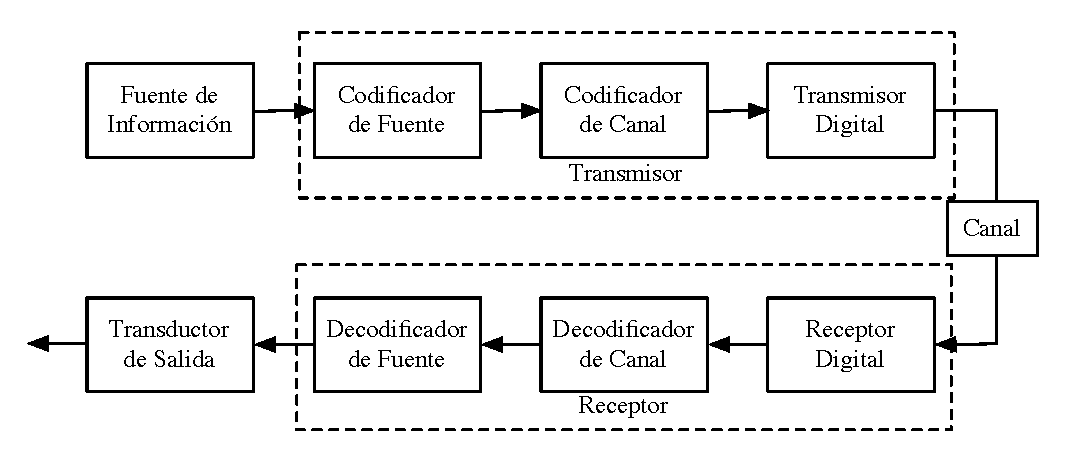
\includegraphics[width=0.95\linewidth]
{introduccion/figuras/fig01-01.pdf}
\caption{Modelo de un sistema de Comunicación Digital I}
\label{fig01-01}
\end{figure}
\end{lstlisting}
%\end{micuadro}

Y el resultado se muestra en la \autoref{fig01-01}.

%
\begin{figure}[htbp]
\centering
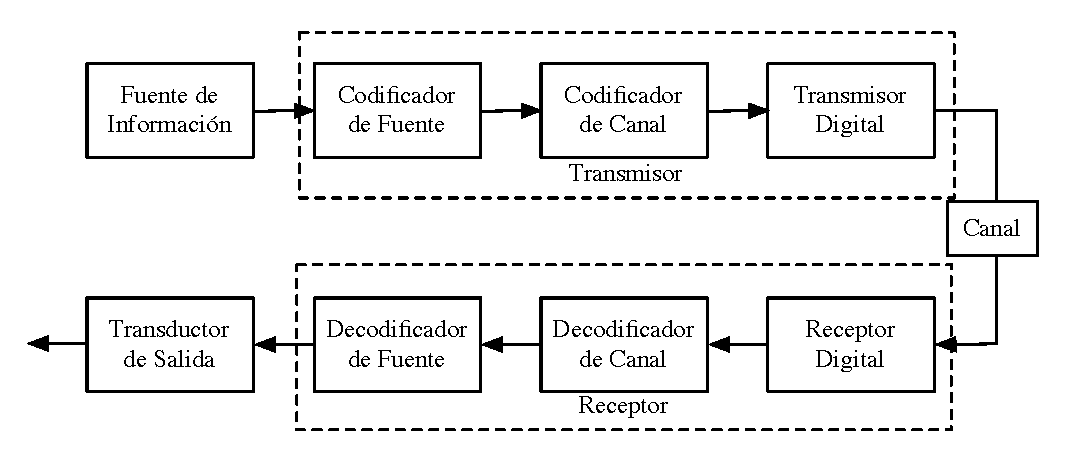
\includegraphics[width=0.95\linewidth]{introduccion/figuras/fig01-01.pdf}
\caption{Modelo de un sistema de Comunicación Digital I}
\label{fig01-01}
\end{figure}
%

Para incluir una tabla utilizamos las instrucciones siguientes:
%\nopagebreak 
\begin{lstlisting}[language=,caption={Inclusión de una tabla}, breaklines=true, label=prg01-02]
\begin{table}[htbp]
	\ttabbox
	{\caption{Tipos de transmisión y frecuencia central} 
	\label{tab2_1}}
		{
		\begin{tabular}{c c}
		\hline
		\rule[-8pt]{0pt}{22pt}{\bfseries{Tipo de Transmisión}}&
		 {\bfseries{Frecuencia central de transmisión}} \\
		\hline
		\rule{0pt}{14pt}Modem & 100-1800 Hz \\
		Radio AM & 530-1600 kHz \\
		Radio FM & 88-108 MHz \\
		Televisión & 178-216 MHz \\
		Telefonía móvil & 850 MHz-1,8 GHz \\
		Redes inalámbricas &  $2,4$ GHz \\
		Fibra óptica & $2\cdot 10^{14}$ Hz \\
		\hline
		\end{tabular}
		}
\end{table}
\end{lstlisting}

Y el resultado se muestra en la \autoref{tab2-1}.

\begin{table}[htbp]
	\ttabbox
	{\caption{Tipos de transmisión y frecuencia central} \label{tab2-1}}
		{
		\begin{tabular}{c c}
		\hline
		\rule[-8pt]{0pt}{22pt}{\bfseries{Tipo de Transmisión}}& {\bfseries{Frecuencia central de transmisión}} \\
		\hline
		\rule{0pt}{14pt}Modem & 100-1800 Hz \\
		Radio AM & 530-1600 kHz \\
		Radio FM & 88-108 MHz \\
		Televisión & 178-216 MHz \\
		Telefonía móvil & 850 MHz-$1,8$ GHz \\
		Redes inalámbricas &  $2,4$ GHz \\
		Fibra óptica & $2\cdot 10^{14}$ Hz \\
		\hline
		\end{tabular}
		}
\end{table}

Observemos  que en la parte inferior de las figuras y en la superior de las tablas (esta ha sido nuestra elección), se colocan textos explicativos sobre las mismas. El formato de este texto se logra mediante una sentencia facilitada por el paquete que se carga mediante el comando \comandos{usepackage}{caption}. El resto de paquetes utilizados realizan diversas tareas como, por ejemplo, \comandos{usepackage}{longtable}, que permite que una tabla se extienda a través de más de una página.

\subsection{Hiperenlaces}
Un primer paso a la hora de crear un documento es generar una versión en formato electrónico del mismo. Hemos decidido que ese formato sea \ttcolor{pdf} . En un formato pdf existe la posibilidad de crear hiperenlaces que facilitan la navegación a lo largo del mismo. Por ejemplo, el índice en un libro en formato pdf se generará, con la propuesta que hemos realizado, creando enlaces a las diversas partes del mismo. O bien, cuando nos referimos a una figura o tabla, es muy útil la existencia de esos enlaces al lugar exacto en el que se encuentra la figura o tabla.  El paquete responsable de realizar todas estas tareas se denomina \ttcolor{hyperref} y las sentencias que siguen a su carga realizan diversas tareas que pueden consultarse en la extensa documentación que lo acompaña. Sobre la línea 110 de \ttcolor{libroTipoETSI.tex} encontrará que puede modificar el color del enlace, puesto a negro por defecto.
% Por ejemplo, no habrá que olvidarse sustituir el literal \ttcolor{F. Javier Payán Somet y Juan José Murillo Fuentes} por el nombre del autor correspondiente.

\subsection{Tabla de contenido}
La generación de la tabla (o tablas) de contenido de un texto suficientemente largo suele ser una tarea sumamente laboriosa. \LaTeX\ facilita enormemente este trabajo mediante un conjunto de paquetes y comandos que se agrupan bajo el apartado genérico denominado TOC (Table Of Contents). En otra sección de este capítulo explicaremos cómo y dónde se incorporará esta tabla de contenidos. En este apartado nos centramos en explicar algunos aspectos de cómo se construye la principal tabla de contenidos, que denominamos  \ttcolor{Índice}.

Nuestra primera decisión fue establecer que en el índice deben aparecer hasta los apartados que hemos denominados \ttcolor{subsubsecciones}, lo que se logra mediante el \ttcolor{\{3\}} del comando \comandos{setcounter}{tocdepth} en \ttcolor{libroETSI.sty}. El formato de cada uno de los apartados se logra con el conjunto de sentencias que siguen y tienen una estructura bastante autoexplicativa. También hemos propuesto que no aparezcan los habituales puntos que existen entre el texto y el número de página correspondiente de muchos índices, ajustando a \ttcolor{10000} el parámetro \ttcolor{\textbackslash@dotsep}. 

Nuestra siguiente decisión afecta a la manera en la que hemos querido que aparezcan en el índice los índices del texto, valga la redundancia. No es trivial pero, básicamente, hemos definido dos listas, una para los elementos que aparecen antes del Índice General y otra para los  que aparecen después, al fina del texto, que se corresponden aproximadamente a lo que hemos denominado \ttcolorc{frontmatter} y \ttcolorc{backmatter}, respectivamente. Si no se desea cualquier índice, basta con comentar la línea correspondiente.

\subsection{Formatos de títulos, páginas y cabeceras y pies de páginas}
El aspecto de un libro está básicamente definido por el formato que se ha elegido para los diferentes títulos de las partes que lo constituyen, el formato de las páginas y qué queremos que aparezca en las cabeceras y pies de páginas del mismo. Todo esto se ha conseguido utilizando un paquete desarrollado por el español Bezos denominado \ttcolor{titlesec}, que se carga en nuestro fichero mediante la instrucción \comandos{usepackage[noindentafter, pagestyles,...]}{titlesec}.

El paquete nos permite definir los distintos tipos de páginas, de acuerdo con las instrucciones que se proporcionan en el mismo. Por ejemplo, con \comandos{newpagestyle}{esitscCD} creamos la página habitual en la mayor parte del texto, formada por el número en la parte exterior de la misma, en las páginas pares el nombre del capítulo en el que estamos y en las impares el nombre de la sección. Estos elementos se colocan encima de una raya horizontal que se ha definido previamente, tanto en su grosor como en su longitud.

Una vez definidos las diferentes tipos de páginas podemos definir, por ejemplo, que nuestra página por defecto será \ttcolor{esitscCD}, con la instrucción \comandos{pagestyle}{esitscCD}. Si queremos que una página determinada en un punto concreto sea diferente, si suponemos que, por ejemplo, el estilo de página \ttcolor{otroestilo} ha sido definido, basta situar la instrucción \comandos{thispagestyle}{otroestilo} en el punto deseado. Un ejemplo podemos encontrarlo en la manera que logramos que los capítulos empiecen siempre en páginas impares. Con ese fin, se utiliza el estilo de página \ttcolor{empty} en caso de que sea necesario.

Por último, el paquete \ttcolor{titlesec} nos permite definir cómo queremos que sean los titulares que usaremos en nuestros textos. Así,  la instrucción \comandos{titleformat}{\textbackslash section ...} establece que nuestras secciones estarán numeradas al nivel de capítulo, con el número de la sección fuera de margen \ttcolor{hang}, y con unas determinadas separaciones del texto, establecidas a través del comando \ttcolorc{titlespacing}. 

En todo caso, estos parámetros no se deberían de tocar, salvo en contadas ocasiones, y por ello se incluyen aquí estos detalles.

\subsection{Teoremas, propiedades, definiciones y demás}
En la escritura de cualquier texto científico los Teoremas, propiedades y demás elementos constituyen una parte muy significativa. Existen, de nuevo, múltiples posibilidades de tratar estos elementos, pero hemos considerado que las facilidades que suministra el paquete \ttcolor{ntheorem}, cargado mediante la instrucción \comandos{usepackage [thmmarks, amsmath, noconfig, hyperref, framed]}{ntheorem} se adapta perfectamente a nuestros gustos y decisiones. Por ejemplo, con el conjunto de instrucciones que se muestran en  el Código \ref{prg01-03}:

\begin{lstlisting}[language=TeX,caption={Teoremas, Lemas,...}, breaklines=true, label=prg01-03]
\theoremnumbering{arabic}
\theoremheaderfont{\aheadteoremas}
\theoremseparator{\hspace{.2em}}
\theorembodyfont{\itshape}
\newtheorem{teor}{Teorema}[section]
\newtheorem{lema}{Lema}[section]
\newtheorem{prop}{Propiedad}[section]
\newtheorem{coro}{Corolario}[teor]
\end{lstlisting}

\noindent hemos definido los Teoremas, Lemas, Propiedades y Corolarios. Centrándonos en los teoremas, las instrucciones anteriores definen que los teoremas estarán referenciados mediante un número \ttcolor{arabic}, con una numeración que será creciente desde la unidad dentro de cada sección de un determinado capítulo, \comandos{newtheorem\{teor\}}{Teorema}\ttcolor{[section]}. La fuente que se utilizará para que aparezca la palabra ``Teorema'' está definida por el comando \ttcolor{\textbackslash theoremheaderfont\{\textbackslash aheadteoremas\}}, el enunciado del teorema se realizará en itálica y para enunciar un teorema y su demostración utilizamos las siguiente instrucciones:

\begin{lstlisting}[language=TeX,caption={Teorema y Demostración}, breaklines=true, label=prg01-04]
\begin{teor}[Teorema de Pitágoras]
En un triángulo rectángulo...
\end{teor}
\begin{proof}
Sea el triángulo ABC...
\end{proof}
\end{lstlisting}

El resultado sería el siguiente:
\begin{teor}[Teorema de Pitágoras]
En un triángulo rectángulo...
\end{teor}
\begin{proof}
Sea el triángulo ABC...
\end{proof}

Podemos observar que al finalizar la demostración hemos incluido el símbolo $\blacksquare$. De manera análoga, están definidas las restantes entidades, incluyendo el comando que nos permite escribir los cuadros de elementos de la programación.

\subsection{Índices de palabras y glosarios}
Con los paquetes index y glossaries podemos incluir índices de palabras y listas con definiciones, ya sea de acrónimos u de otro tipo. Por ejemplo, se podría usar también para definir magnitudes o la notación utilizada.
 
%http://en.wikibooks.org/wiki/LaTeX/Indexing
\subsubsection{Índices de palabras}
\index{Indice de palabras@Índice de palabras!index}%\index{\'Indice de palabras!index}\index{Índice de palabras!indexit}
Para construir un índice de palabras\index{Indice de palabras@Índice de palabras}, como el que puede encontrar al final de este texto, se incluye el paquete \comandos{usepackage}{imakeidx} con algunas opciones. Para incluir una palabra  en el índice utilizamos   \comandos{index}{palabra} justo detrás de la palabra que queramos indexar. Si queremos agrupar en un grupo diferentes subpalabras \index{Indice de palabras@Índice de palabras!subpalabra}, utilizamos \comandos{index}{palabra!subpalabra}. Es importante no olvidar ejecutar \ttcolor{makeindex}, al igual que ejecuta latex o bibtex para componer el texto o generar la bibliografía. Otro detalle importante es poner los índices con mayúsculas o con minúsculas, pero todos iguales. De esta forma, cuando se genere el índice de palabras no queden algunas con la primera letra en mayúsculas y otras no. Por último, con las instrucciones de compilación que se detallan un poco más adelante, las palabras en español que empiecen por tilde se indexan al final. Para evitarlo, y que aparezcan en su sitio, tiene que escribir primero la palabra sin tilde seguida de arroba y la palabra con tilde, como por ejemplo \ttcolorc{index\{Indice de palabras@Índice de palabras\}}. 

\subsubsection{Glosario}
Un glosario con acrónimos u otros términos se realiza en este texto utilizando\\
 \comandos{usepackage [acronym]}{ glossaries}. 
 Para definir un acrónimo, basta con incluir antes del comienzo del documento una línea del tipo:\\
 \comandos{newacronym[type=main]\{etiqueta\}\{acrónimo\}}{nombre completo}, 
 \\
 como por ejemplo\\
 \comandos{newacronym[type=main]\{ETSI\}\{ETSI\}}{Escuela Técnica Superior de \\Ingeniería}. 
 \\
 En esta orden el primer argumento es el identificador o etiqueta, el segundo es el acrónimo o abreviatura y el tercero es el nombre completo al que hace referencia el acrónimo o abreviatura. Para utilizar luego la abreviatura o acrónimo, y se pueda luego generar un índice que indique en qué página se ha usado, se utiliza \comandos{gls}{etiqueta}. 

\subsubsection{Compilación de índices de palabras y glosarios}
Existen distintos comandos para generar el índice y el glosario. Puede utilizar los que estime oportunos. Aquí se ofrece una solución para realizarlo.

El comando más usado es \ttcolor{makeindex}. Habría que llamar dos veces a este comando, con distintos argumentos, si se incluye el glosario además del índice. En Macintosh si utiliza el comando \ttcolor{lualatexmk}, uno de los engines de TeXShop\index{engine}, el índice de palabra y el glosario se generarán de forma automática. 
%Puede usar Texindy\index{Texindy} para una presentación del índice de palabras con otra presentación.

En Windows, tendrá que ejecutar PDFLatTeX ó LatexMk, luego tendrá que ejecutar makeindex tal cual para generar el índice de palabras. Para generar el glosario tendrá que definir un comando de usuario, tal como sigue. Vaya al menú `Usuario', en texmaker, y allí a `Comandos de Usuario' y dentro de este a `Editar Comandos de Usuario'. En cualquiera de los comandos defina uno nuevo con el título que quiera, por ejemplo glosario, y en el campo comando, incluya la siguiente línea\footnote{Si usase el texmaker en Mac-OS tendría que pulsar el asistente para seleccionar makeindex. Aparecería en el campo comando algo así como \ttcolor{''makeindex'' \%.idx}, donde el asistente habrá encontrado la carpeta donde está el comando makeindex. Sustituya el final, \%idx, por  -s \%.ist -t \%.glg -o \%.gls \%.glo, de forma que el campo comando quede como sigue:
 \ttcolor{''/usr/texbin/makeindex'' -s \%.ist -t \%.glg -o \%.gls \%.glo}}

Una vez definido este comando de usuario, ejecútelo, y vuelva a ejecutar PDFLaTeX o LatexMk.

\section{Antes del documento}
Antes de empezar la edición del documento, además de cargar los ficheros de estilos \ttcolor{LibroETSI.sty} y \ttcolor{edicionLibro.sty} (o el correspondiente al documento),  hemos creído necesario realizar una serie de operaciones que faciliten nuestro trabajo o lo configuren de una determinada manera. %Además, hay que incluir la portada.

\subsection{Fichero de notación: notacion.sty}
Hemos considerado interesante incluir un fichero de notaciones que son de amplia utilidad dentro del área de conocimiento de los autores. Su uso es completamente opcional pero se ha utilizado ampliamente en la elaboración de este texto. Simplifica enormemente la escritura hacer uso de ficheros de este tipo y prácticamente cada autor utiliza el suyo propio.

Como ocurría con el fichero \ttcolor{LibroETSI.sty}, es necesario que se cargue, incluyendo la instrucción \comandos{usepackage}{notacion} al comienzo del fichero principal. Puesto que su uso resulta evidente, no hemos considerado necesario realizar una documentación precisa sobre el mismo más allá de los propios comentarios que acompañan las definiciones del fichero, y que el lector puede consultar abriéndolo. Nótese que existe además una carpeta con este nombre. En esta carpeta se ha incluido un ejemplo de notación que podría ponerse al comienzo de un documento. Sobre este documento, se puede añadir o quitar lo que se desee.

\subsection{Fuente del texto}
Las instrucciones incluidas en el código \ref{prg01-05} y que pertenecen al fichero \ttcolor{LibroETSI.sty} 
 se pueden modificar para cambiar la fuente del texto.  En primer lugar, debemos actuar de forma diferente si queremos utilizar la fuente Minion Pro o no.  Si hemos definido como \ttcolor{true} el parámetro correspondiente, en el caso que estemos compilando con \LaTeX\ no debemos hacer nada. Sin embargo, en el caso de utilizar \LuaLaTeX\ debemos declarar que la fuente va a ser Minion Pro y modificar ligeramente su tamaño.
 
Si no vamos a utilizar una fuente Minion Pro, en el caso de \LuaLaTeX\ se puede utilizar para el texto cualquier fuente OTF o TTF que el usuario posea de forma legal, y se encuentre instalada, lo que depende del sistema operativo (SO) utilizado. En nuestro caso, observad que hemos utilizado una fuente Time New Roman  pues suele estar instalada en la mayoría de los SO. Se proponen asimismo un par de alternativas si prefiere otras fuentes.
 
El código incluido detecta si se no se está utilizando \LuaLaTeX\, en cuyo caso se usa una fuente equivalente a una Times, cargada mediante el comando estándar \comandos{usepackage}{tgtermes}. Hay otras opciones comentadas, y se pueden buscar otras fuentes. 
 
\begin{lstlisting}[language=,caption={Fuente del texto}, breaklines=true, label=prg01-05]
%:Para modificar fácilmente la fuente del texto. 
\makeatletter
\ifdtsc@Minion % Queremos utilizar la fuente Minion y lo hemos declarado al principio
	\ifluatex
		\setmainfont[Renderer=Basic, Ligatures=TeX,	% Fuente del texto 
		Scale=1.01,
		]{Minion Pro}
   		% En este caso conviene modificar ligeramente el tamaño de las fuentes matemáticas
		\DeclareMathSizes{10}{10.5}{7.35}{5.25}
		\DeclareMathSizes{10.95}{11.55}{8.08}{5.77}
		\DeclareMathSizes{12}{12.6}{8.82}{6.3}
	\fi
\else
	\ifluatex
		% Para utilizar la fuente Times New Roman, o alguna otra que se tenga instalada
		\setmainfont[Renderer=Basic, Ligatures=TeX,	% Fuente del texto 
		Scale=1.0,
		]{Times New Roman}
%		\setmainfont[Renderer=Basic, Ligatures=TeX,	% Fuente del texto 
%		]{Adobe Garamond Pro}
%		\setmainfont[Renderer=Basic, Ligatures=TeX,	% Fuente del texto 
%		]{Palatino LT Std}
	\else
		\usepackage{tgtermes} 	%clone of Times
		%\usepackage[default]{droidserif}
		%\usepackage{anttor} 	
	\fi
\fi
\makeatother
\end{lstlisting}

Si se intenta utilizar una fuente que no está instalada (dentro del sistema operativo) la compilación con \LuaLaTeX\ daría error. Si se instala una nueva fuente y se desea utilizar, se puede tratar de modificar las líneas de código que se suministran como ejemplo. La primera vez que se utilice esa nueva fuente, \LuaLaTeX\ tardará algo más en compilar pues necesita generar una serie de ficheros internos.

La principal ventaja en el uso de \LuaLaTeX\ la encontramos en la facilidad para utilizar diferentes fuentes en diferentes lugares y con diferentes características (tamaño, color, etc) muy fácilmente configurables. Puede ser interesante leer el fichero \ttcolor{fontspec.pdf} para conocer cómo se realizan estos cambios. 

En caso de utilizar el motor pdfLatex, la elección más sencilla se realiza como hemos dicho mediante paquetes específicos tales como \comandos{usepackage}{tgtermes}. Puede consultarse la dirección \url{http://www.tug.dk/FontCatalogue/alphfonts.html} para conocer las posibilidades más habituales. 

Por último: como ya hemos dicho, todo lo anterior únicamente afecta a la elección de las fuentes del texto. La elección de las fuentes matemáticas (texto dentro de matemática, símbolos, letras griegas, etc) se controla de manera completamente diferente mediante paquetes específicos. En el \autoref{estilo} volveremos sobre este asunto. En concreto, observar que en el caso de compilar con la opción \ttcolor{Minion=true} y existir el fichero de estilo \ttcolor{MinionPro.sty} (no confundir con la fuente Minion Pro; si no existiera el fichero, aparecería un error), se propone el uso de la fuente Minion Pro como fuente matemática, junto con los símbolos de la fuente MnSymbol. En caso contrario, se hará uso de una fuente Times (en realidad, de una extensión de la misma). 

No todas las fuentes pueden usarse como fuentes matemáticas y en la dirección \url{http://www.tug.dk/FontCatalogue/alphfonts.html} se encuentran recogidas las que si tienen soporte matemático. Es importante señalar además que no todas las combinaciones de fuente de texto y fuente matemática son tipográficamente adecuadas. 

\subsection{Cubierta y primeras páginas}
Se ha diseñado esta plantilla para que tome una imagen de fondo y a partir de ésta se incluyan los datos de título, autor, etc, para generar la portada del documento. La portada propuesta es distinta para proyectos fin de carrera y similares que para libros o tesis. Todo esto se ha hecho diseñando una serie de funciones que las generan, tomando los datos que se definen en la cabecera del fichero principal. Así, en el \ttcolor{libroTipoETSI.tex}, se puede definir el título de la obra, el autor, etc. En el caso de \ttcolor{pfcTipoETSI.tex} y \ttcolor{tesisTipoETSI.tex}, se puede definir además el director, el tipo de proyecto (máster, grado y carrera), y otros parámetros. Las imágenes de fondo de la cubierta también se llaman desde este fichero, así como la imagen al pié de la hoja interior con el título y autor de la obra (para libros). La imagen central de la cubierta está en la carpeta figuras, con nombre \ttcolor{imagenLibro.png}. Puede incluir la imagen deseada en esta carpeta salvándola con este mismo nombre. Preste atención a que el formato es rectangular. Para introducir la imagen del logo del departamento en el proyecto fin de carrera/grado/máster, puede retocar la imagen de fondo, cortando el logo existente e insertando el deseado. Estas imágenes están en la carpeta figuras. 

Para cambiar cualquier otro aspecto, tales como el tamaño de la figura de la cubierta ó los créditos de la cubierta, tendrá que modificar el fichero \ttcolor{edicionLibro.sty} en este caso de un libro. 

%En el ejemplo que se presenta para libros, el latex toma una imagen de fondo, y otra, imagenLibro.png,  de la portada para incluir además de los datos de título y autores, definidos al comienzo del fichero \ttcolor{portadaLibro.tex}, una imagen superpuesta representativa de la temática del texto. Los autores pueden cambiar esta imagen fácilmente por otra acorde a su texto.

%Sería interesante poner algo sobre citas

\endinput
%Introducción
%
\chapter{Descripción del hardware}\label{chp-02}
%
\chapter{Desarrollo de placa de conexiones}\label{chp-03}

\lettrine[lraise=-0.1, lines=2, loversize=0.2]{P}ara simplificar todas las conexiones internas
dentro de la caja y posibilitar ciertas funciones especificadas, se crea una placa electrónica
donde se conectan todos los dispositivos. De este modo se consigue simplificar el montaje y la
posible actualización del sistema, ya que todas las conexiones internas desaparecen por completo.
Además, para favorecer el orden de los cables dentro de la caja se crea una segunda placa más básica
cuya única función es agrupar todas las conexiones existentes en la tapa. Se conocerá como placa \textit{Fondo}
a la placa general y placa \textit{Tapa} a la superior.

\section{Software utilizado. KiCAD.}

Para la realización de la placa se ha utilizado el paquete de software KiCAD. Se trata de un software 
libre bajo licencia GNU General Public License, lo que permite su uso sin coste para el proyecto. KiCAD
es un paquete de software orientado hacia el diseño electrónico (EDA por sus siglas en inglés: Electronic
Design Automation) y consta de diversas aplicaciones que permiten realizar todo el trabajo.

\begin{figure}[hbtp]
    \centering
    
\includegraphics[width=\textwidth/2]{03-placa/01-KiCad-Logo.png}
    \caption{Logo de KiCAD}
    \label{fig:figura31}
    \end{figure}

Por un lado cuenta con \textit{eeschema}, un editor de esquemas electrónicos donde se puede plantear
la lógica de las conexiones de un modo abstracto. Por otro, se encuentra con \textit{pcbnew}, un editor
de circuitos impresos. A partir de un esquemático creado se pasa a un circuito impreso de modo fácil y
siendo modificable siempre que sea necesario.

\section{Niveles lógicos de tensión}

En primer lugar, el proyecto cuenta con dispositivos que funcionan a distintos niveles de tensión, por 
lo que se tiene que plantear las transformaciones a realizar. Los dos principales niveles de tensión 
son los 5V a los que funciona el Arduino y los 24V a los que funciona el motor y la controladora del 
robot. Por otra parte, también se cuenta con el nivel lógico de 1.5V del calibre digital.

El sistema se alimenta con 24V provenientes de la controladora y pasa a 5V mediante el convertidor
externo con el que se cuenta, por lo que con obtener dichas conexiones del propio sistema ya se dispone
las dos líneas. Sin embargo, en el caso de los 1.5V éstos deben ser generados dentro de la placa como
se verá en la sección correspondiente más adelante.

\section{Señales digitales en 24V y en 5V}

El sistema cuenta con cuatro salidas digitales que deben estar representadas tanto en 24V como en 5V
para que tanto el Arduino como la controladora conozcan de modo inequívoco el modo en el que se encuentra
el sistema. Estas señales son:
\begin{itemize}
    \item Microcontrolador (MICRO). '1' si el microcontrolador se encuentra desactivado y '0' si está operativo.
    \item Local/Remoto (LR). '1' si el sistema funciona en modo remoto y '0' si funciona en modo local.
    \item Emergencia (EMER). '1' si el sistema requiere una parada de emergencia.
    \item Sensor Fotoeléctrico (FOTO). '1' si hay una pieza detectada por el sensor.
\end{itemize}

Además, se cuenta con dos entradas digitales que deben ser capaces de mover el motor en el caso de que el
sistema se encuentre funcionando sin microcontrolador. Para ello estas señales deben actuar sobre los
pines de dirección del L298N. Estas dos señales son:
\begin{itemize}
    \item Avance (AVANCE). Actúa sobre el pin IN1 o IN3 del L298N.
    \item Retroceso (RETR). Actúa sobre el pin IN2 o IN4 del L298N.
\end{itemize}

Las señales se generan a 24V por defecto, por lo que es necesario su paso a 5V. Para ello se utilizan
optoacopladores, unos dispositivos que mediante fotodiodos acoplados a fototransistores. En este proyecto
se utiliza el circuito integrado TLP621-4 que cumple dicha función.

\begin{figure}[hbtp]
    \centering
    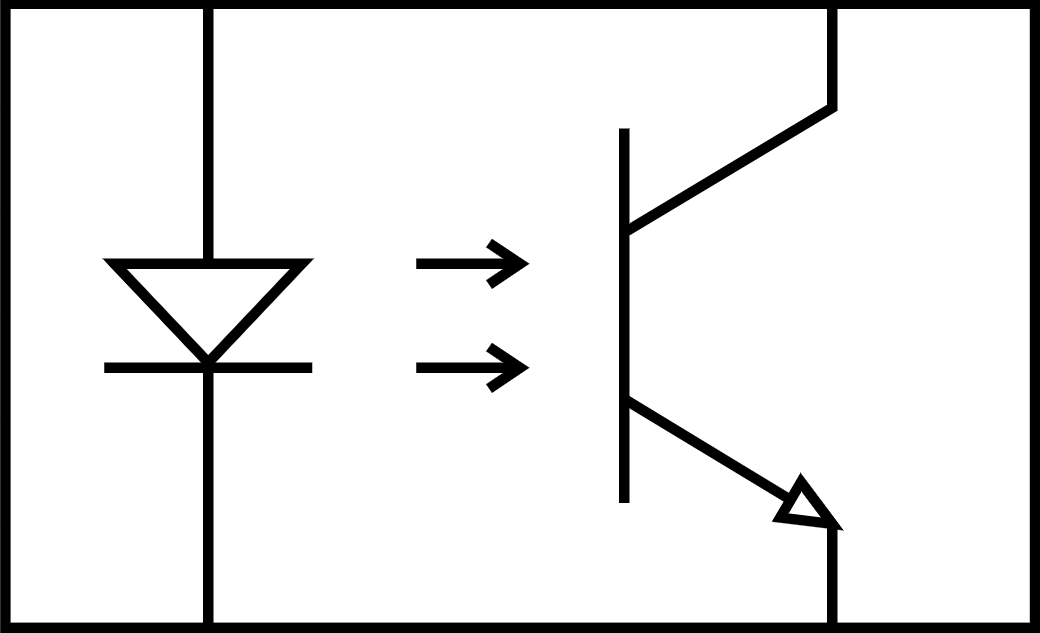
\includegraphics[width=\textwidth/4]{03-placa/02-optoac.png}
    \caption{Ejemplo de optoacoplador}
    \label{fig:figura32}
    \end{figure}

\subsection{Implementación de optoacopladores}

En la figura \ref{fig:figura33} se muestra el circuito empleado. Se utiliza un total de dos TLP621-4 para
tener un total de 8 optoacopladores. Como la tensión máxima que reciben los diodos es de 24V, se colocan
unas resistencias para evitar que se quemen. El valor de las resistencias utilizadas es de 8.2 k$\Omega$,
permitiendo que la corriente directa sea algo inferior a 3 mA. Como caso relevante, en el caso de la parada
de emergencia, la resistencia será de 4.7 k$\Omega$ para que tenga una corriente directa y, una mayor
salida por ello para asegurar que se produzca la parada en caso de ser necesaria.

\begin{figure}[hbtp]
    \centering
    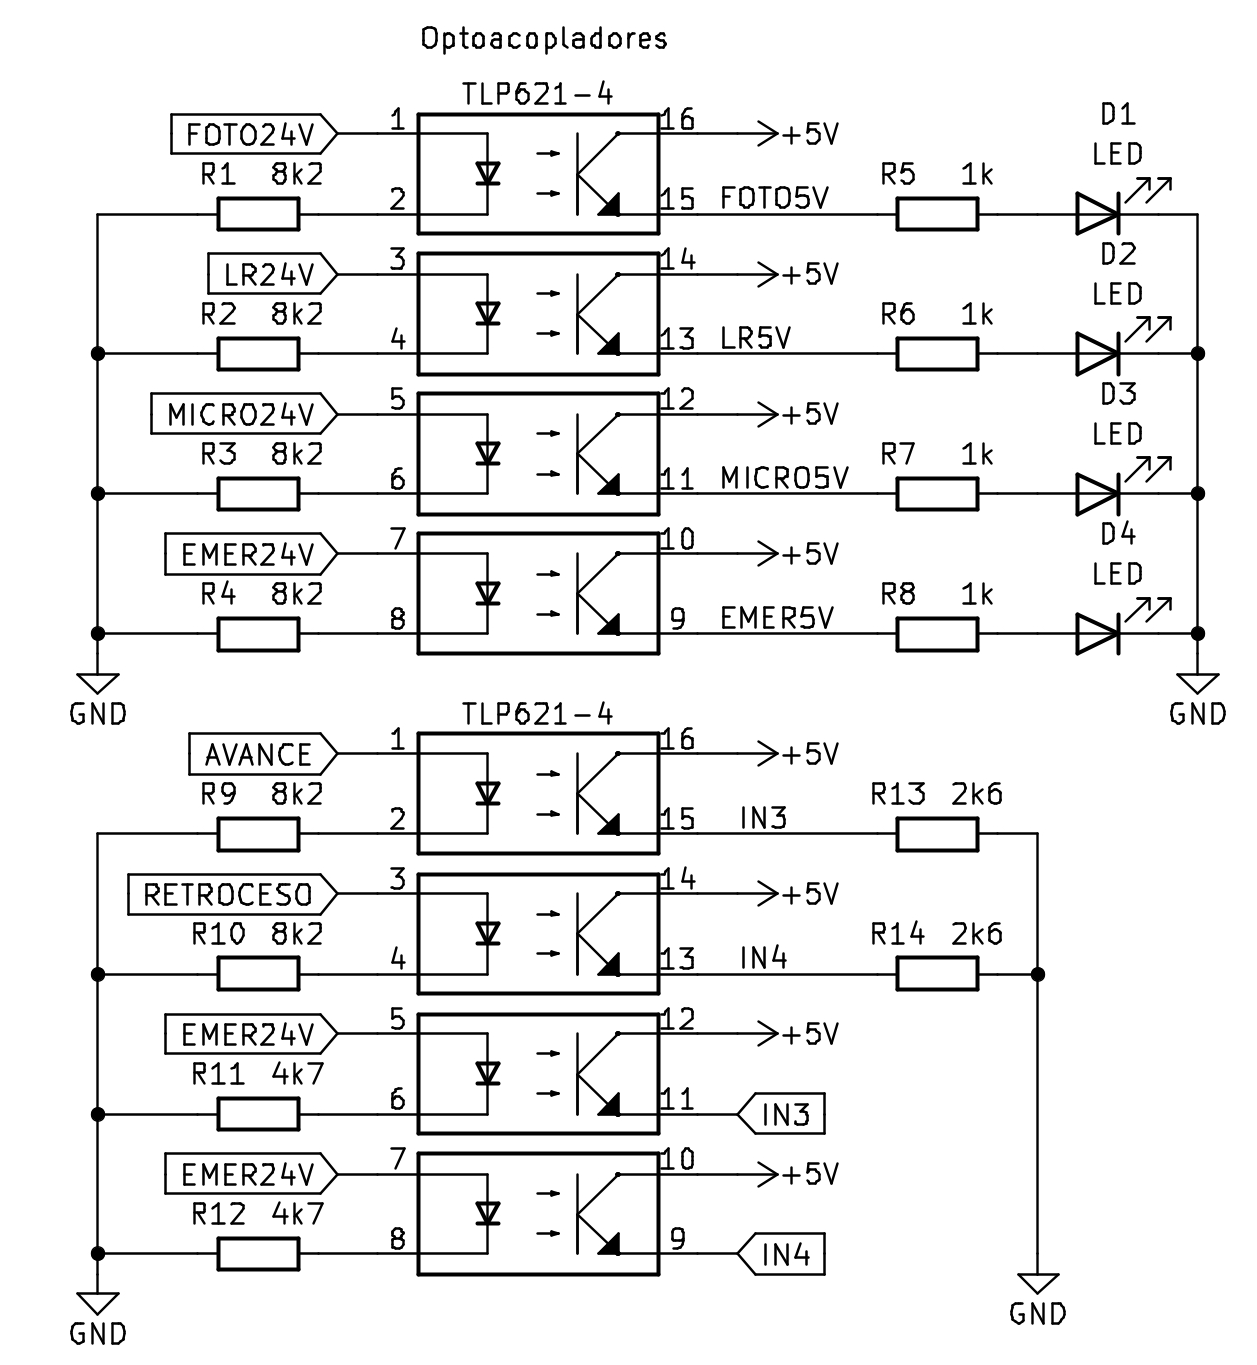
\includegraphics[scale=1.25]{03-placa/03-optoacopladores.png}
    \caption{Implementación de optoacopladores}
    \label{fig:figura33}
    \end{figure}

En el colector de los fototransistores se conectan directamente la línea de 5V para que, en caso de que la
señal correspondiente se active, su equivalente de 5V también lo haga. En las señales FOTO, LR, MICRO y EMER
se les añade un LED a la salida a modo de test para comprobar su funcionalidad, pero no se verán desde fuera
de la caja.


\section{Calibre digital}

\subsection{Alimentación calibre}

Para el funcionamiento del calibre digital, éste debe ser alimentado por una fuente de 1.5V. Como lo que se
dispone en este proyecto es de 5V y 24V lo más sencillo es colocar un divisor resistivo a la línea de 5V y
utilizar un búfer de tensión para mantener dicho nivel lógico estable. Utilizando resistencias lo suficientemente
altas el consumo es despreciable. Por ello se utiliza una resistencia de 39k$\Omega$ y otra de 100k$\Omega$. La 
tensión de salida obtenida será de:

\begin{equation}
    V_{out} = 5V \frac{39k\Omega}{39k\Omega+100k\Omega} \approx 1.4V
\end{equation}

Los 1.4V que se obtienen entran dentro del rango de funcionamiento del calibre utilizando resistencias comerciales,
por lo que el resultado es válido. 

El consumo del divisor resistivo por otro lado será de:

\begin{equation}
    I_{divisor} = \frac{5V}{39k\Omega+100k\Omega} \approx 0.036 mA
\end{equation}

Se puede considerar un consumo despreciable.

Para el búfer de tensión se utiliza un circuito integrado TL082, del cual se utiliza uno de los dos amplificadores
operacionales con el que cuenta. Como resultado se obtiene el circuito de la Figura \ref{fig:figura34}.

\begin{figure}[hbtp]
    \centering
    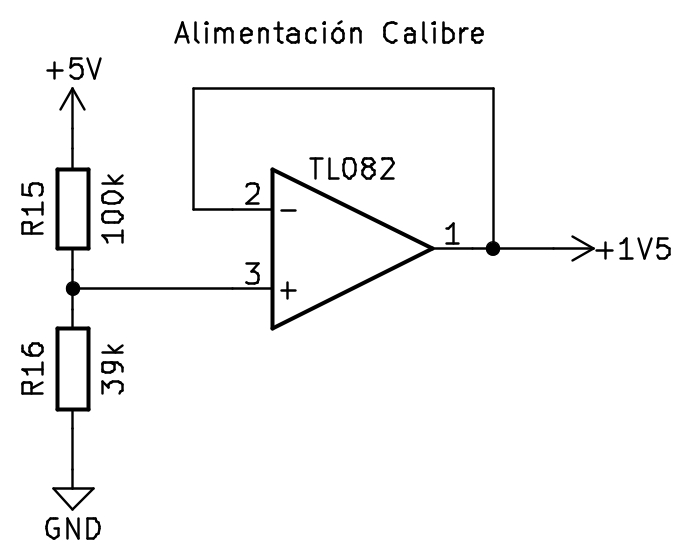
\includegraphics[width=\textwidth/2]{03-placa/04-alimentacion-calibre.png}
    \caption{Alimentación calibre digital a 1.5V}
    \label{fig:figura34}
    \end{figure}

\subsection{Amplificación señales calibre}



\begin{figure}[hbtp]
    \centering
    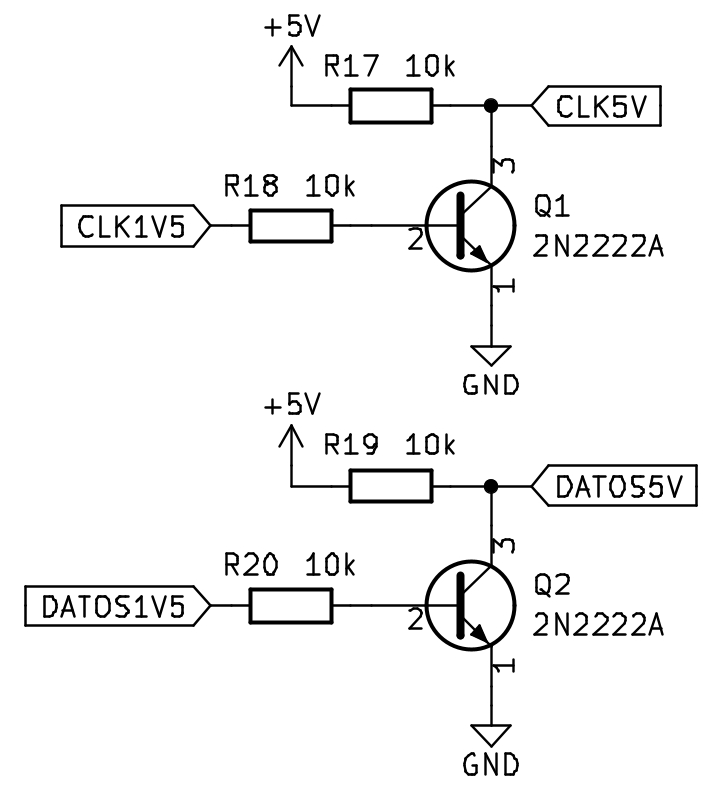
\includegraphics[width=\textwidth/2]{03-placa/05-amplificacion-calibre.png}
    \caption{Amplificación señales calibre digital a 5V}
    \label{fig:figura35}
    \end{figure}




Calibre digital
Tapa

%
\chapter{Planificación de caja}\label{chp-04}

Para que todos los dispositivos que componen el sistema estén bien aislados del exterior
y no haya problemas con las conexiones se planifica una caja estanca. Ésta deberá ser 
accesible para el reemplazo de dispositivos defectuosos y ser replicable. 

Como referencia se toma de una caja de dimensiones 220 x 145 x 80 mm. Para reducir los 
costes, se decide imprimirla en 3D, ya que permite mayor adaptabilidad para colocar 
los lugares donde fijar los diferentes dispositivos. La caja estará dividida en una base y una 
tapa que se unen mediante tornillos y permiten una unión estable.

\section{Base}

La base debe tener las siguientes características:
\begin{itemize}
    \item Permitir fijar y extraer con facilidad todos los dispositivos. 
    \item Orificio para entrada de cables de conexión.
    \item Hueco para conector hembra Ethernet.
    \item Hueco para conector de pines digitales.
\end{itemize} 

Con todo ello se ha diseñado la base que se puede ver en la figura \ref{fig:cajabase}. Se muestra
una imagen de la planta y otra general. Se puede observar que cuenta con distintos orificios en los
que se debe introducir tuercas M3 durante la impresión en 3D para los distintos anclajes de dispositivos
que se comenta a continuación y para la unión con la tapa para que quede estanca la caja.

Además, para el anclaje de los dispositivos sobre la base, se ha diseñado un soporte que va atornillado
a la misma. Para ello, se ha modelado de forma simplificada todos los dispositivos y se ha buscado la 
forma óptima de disponerlos. También se ha tenido en cuenta los cables que van conectados tanto a la 
fuente como al Arduino, modelándolos en el espacio que ocupan hasta que el ángulo de giro es aceptable
para que el cable se pueda colocar de forma holgada y sin tensiones dentro de la caja.
Posteriormente se ha creado el soporte en base a dicha disposición y contando con los orificios de cada
dispositivo. En la figura \ref{fig:ensamblajebase} se puede observar el resultado final de este ensamblaje.

\newpage

\begin{figure}[htpb]% 
    \centering 
    \subfloat[][]{% 
        \label{fig:cajabasevista}% 
        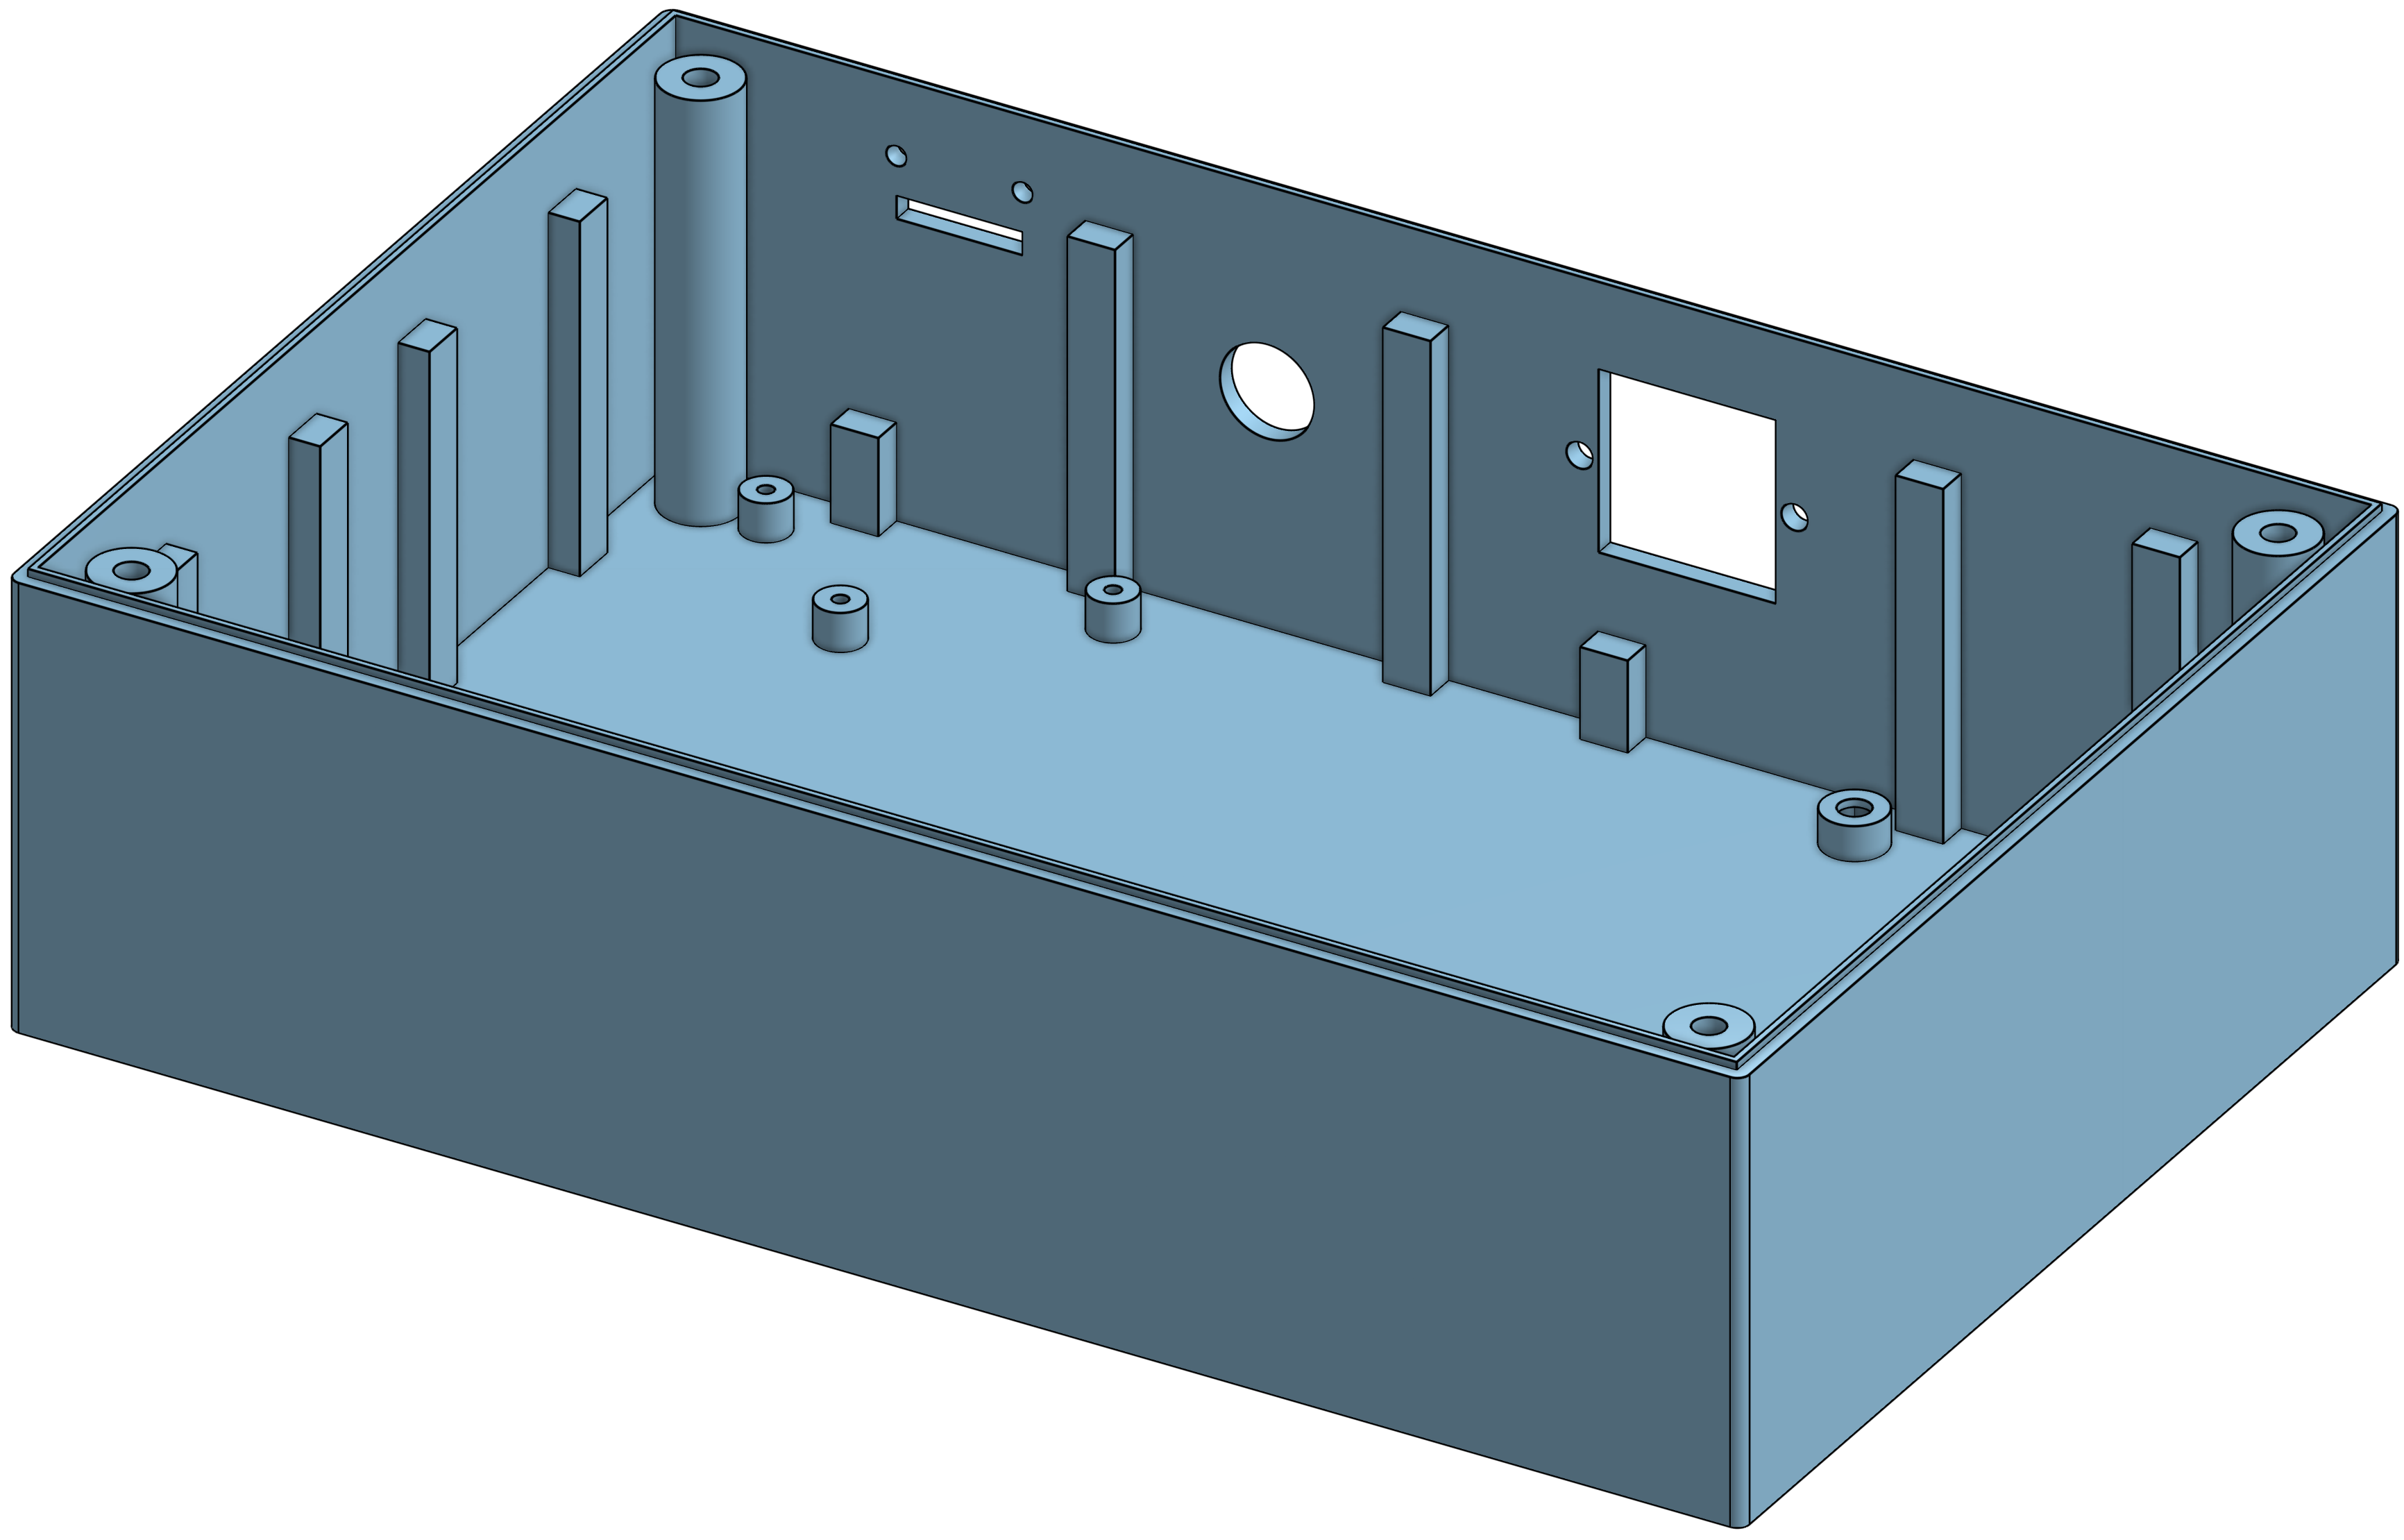
\includegraphics[width=0.5\textwidth]{04-caja/cajabase.png}
    }% 
    \hspace{10pt}% 
    \subfloat[][]{% 
        \label{fig:cajabaseplanta}% 
        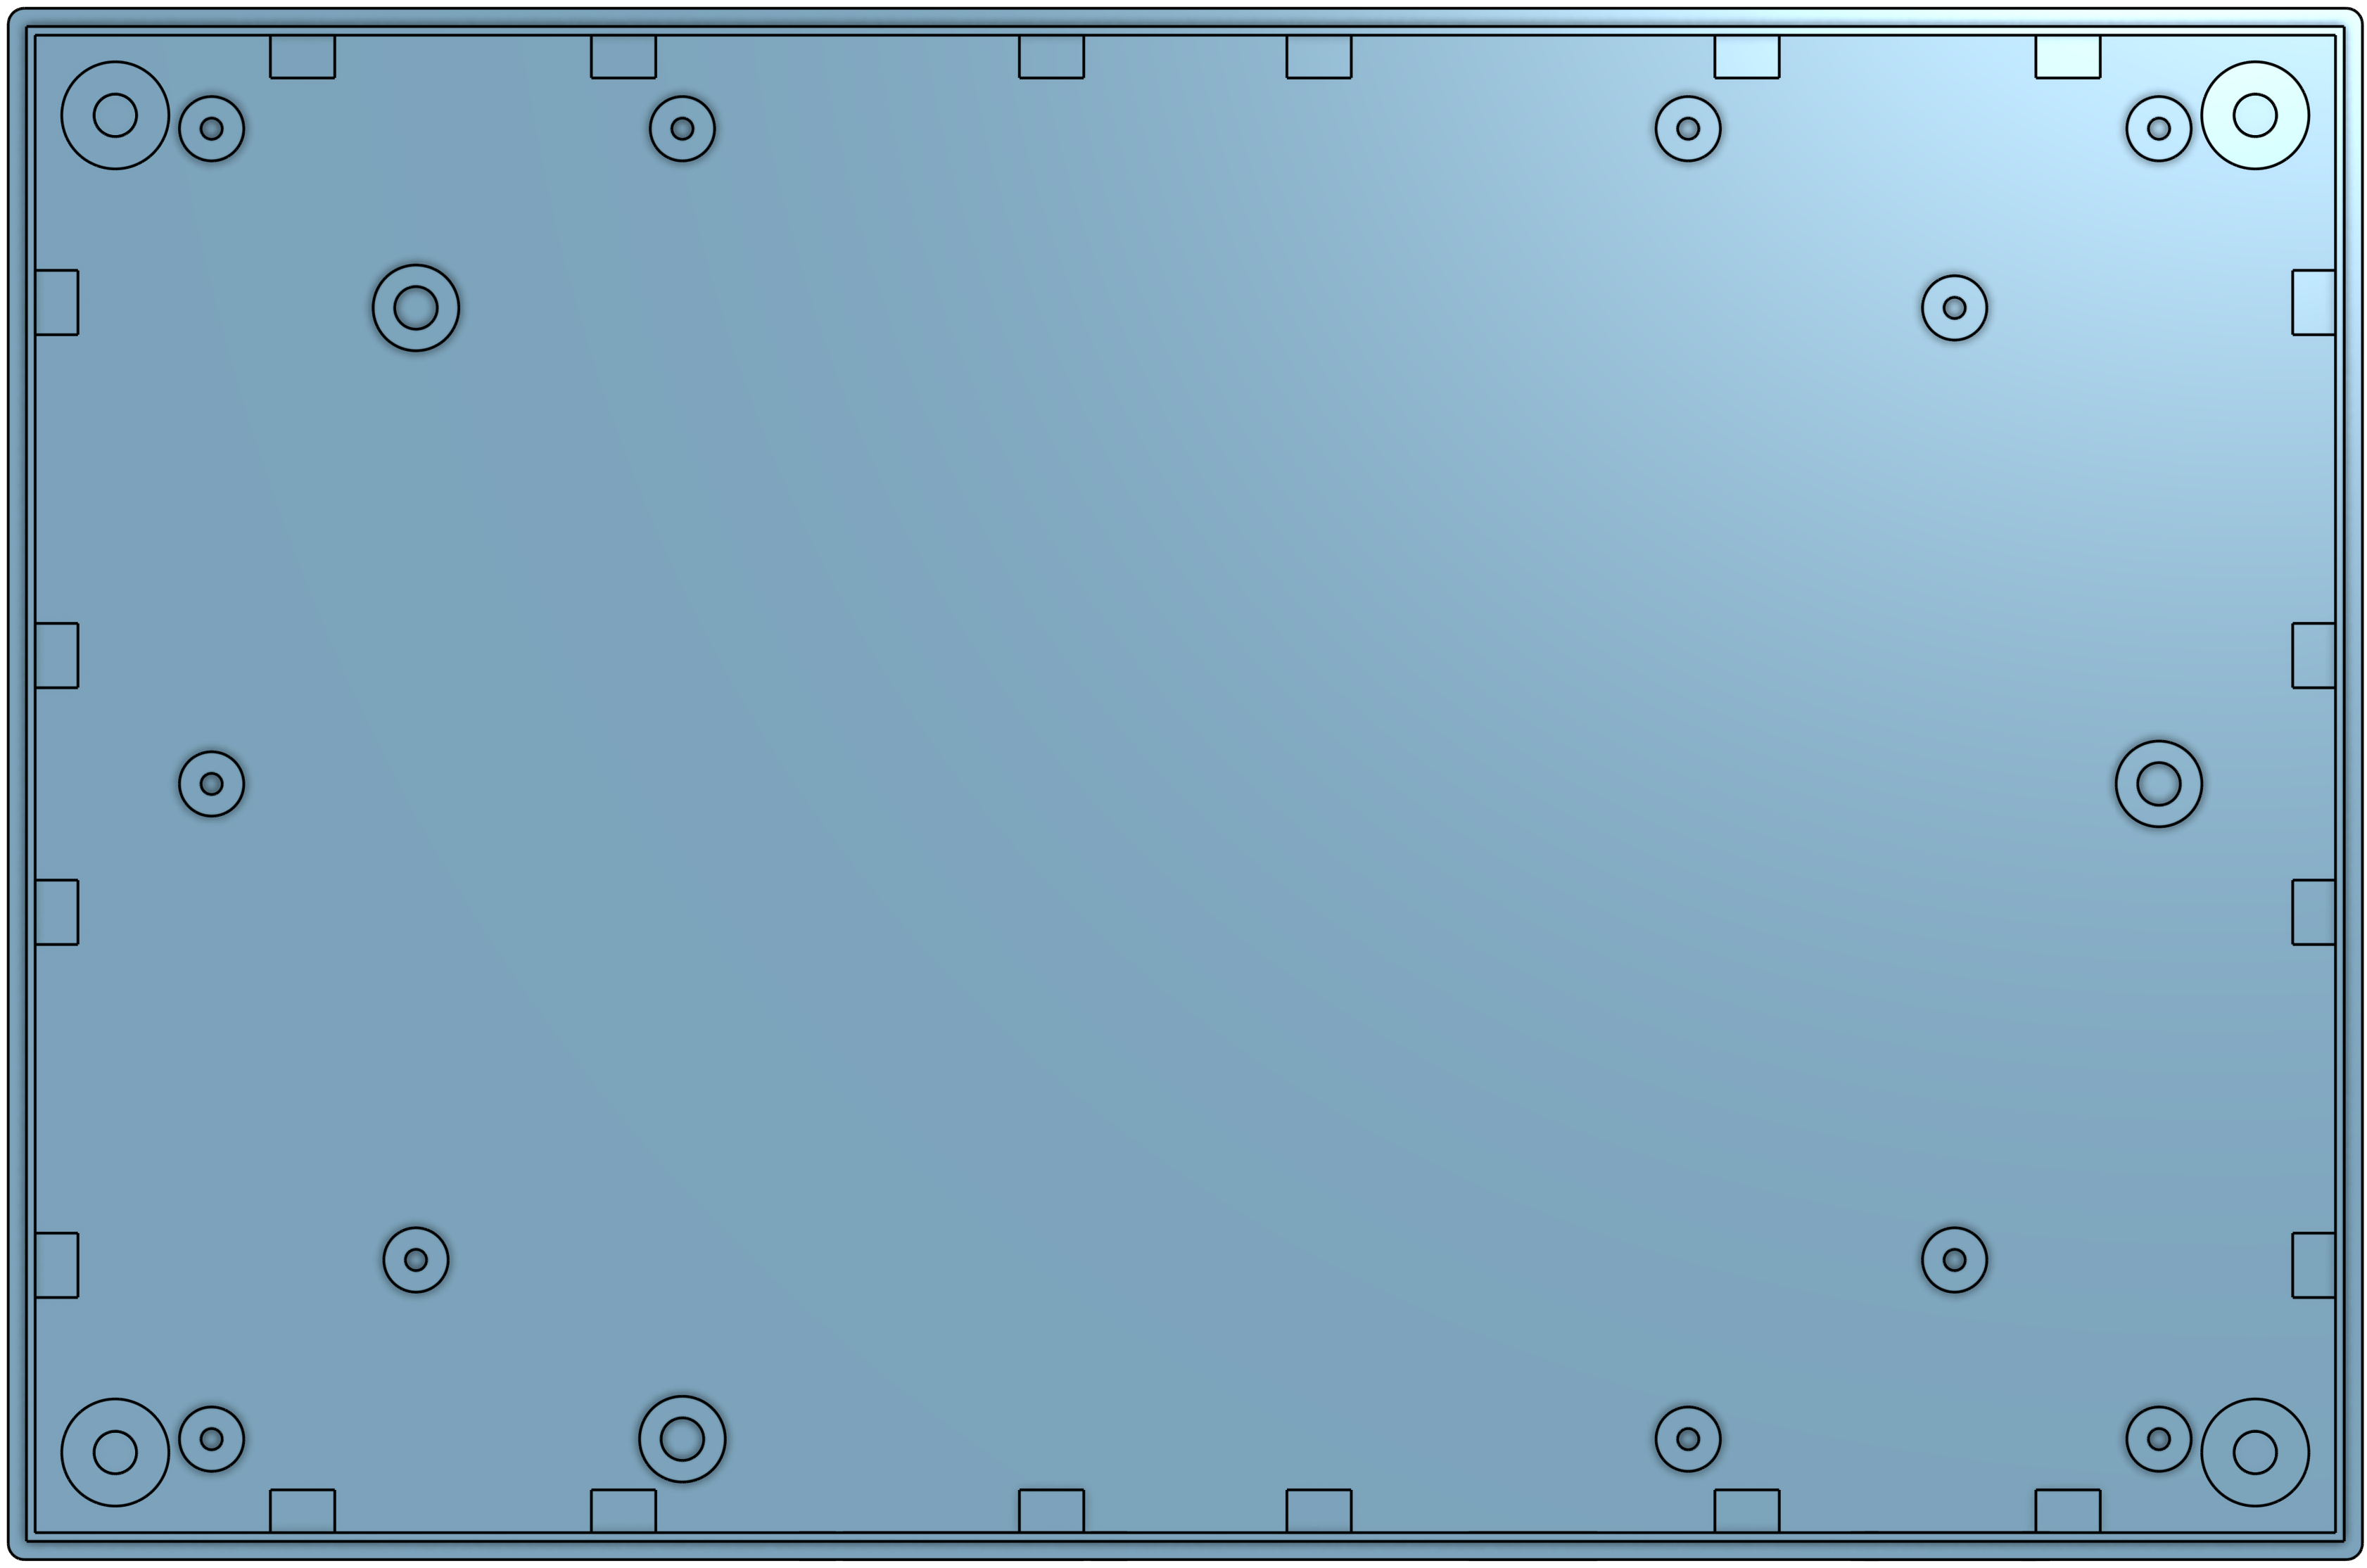
\includegraphics[width=0.5\textwidth]{04-caja/cajabaseplanta.png}
    }
    \caption{(a) Vista general de la base de la caja. (b) Vista de planta de la base de la caja}
    \label{fig:cajabase} 
\end{figure} 


\begin{figure}[hbtp]
    \centering
    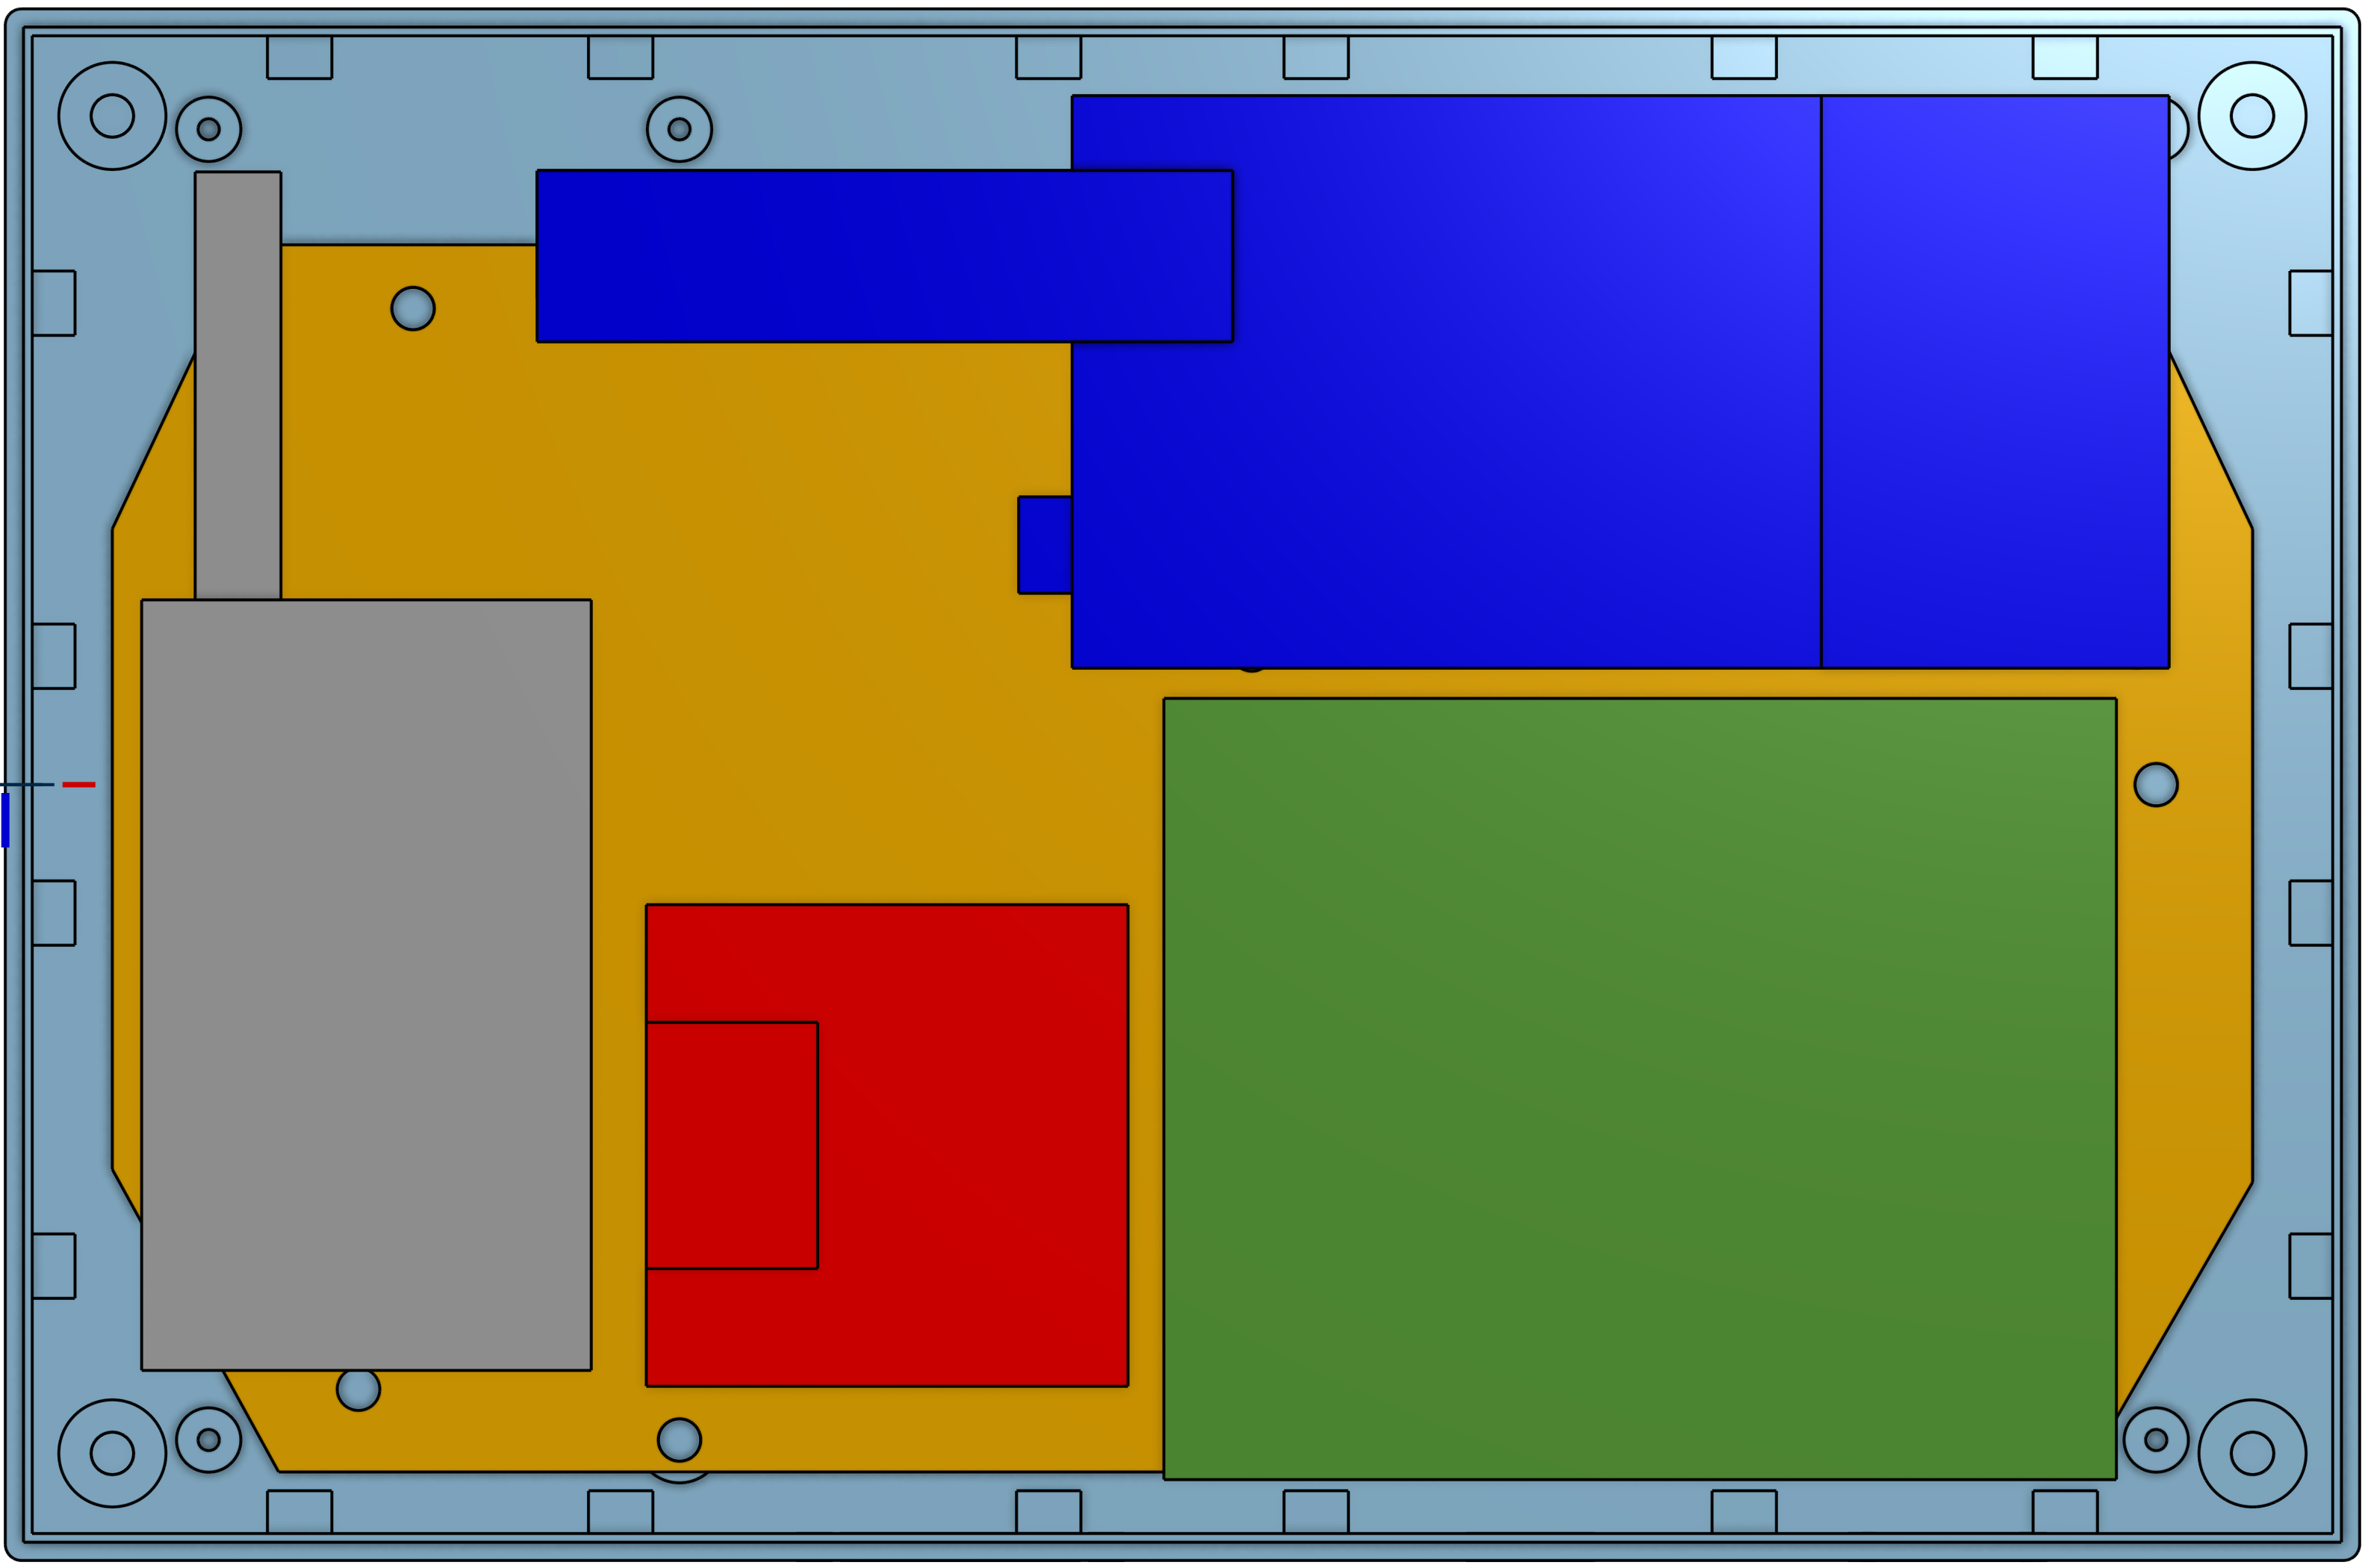
\includegraphics[width=0.5\textwidth]{04-caja/ensamblajebase.png}
    \caption{Ensamblaje de la base con el soporte. Descripción por colores: a) Gris: Fuente. 
    b) Rojo: L298N. c) Azul: Arduino. d) Verde: placa de conexiones. e) Amarillo: Soporte tapa}
    \label{fig:ensamblajebase}
    \end{figure}


\section{Tapa}

La tapa debe ser el soporte para la interfaz humano-máquina y, por ello, sostener todos sus 
dispositivos. Por lo general, todos los dispositivos que van en la tapa son de tamaño reducido,
a excepción de la seta de emergencia, por lo que no hay problemas con su distribución. La seta
de emergencia se ubicará en la esquina superior izquierda, situándose justo encima de la placa
de conexiones del fondo, ya que ésta es la de menor altura. En la figura \ref{fig:cajatapa} se 
muestra la tapa tanto en la planta como en una vista general.

\begin{figure}[h]% 
    \centering 
    \subfloat[][]{% 
        \label{fig:cajatapavista}% 
        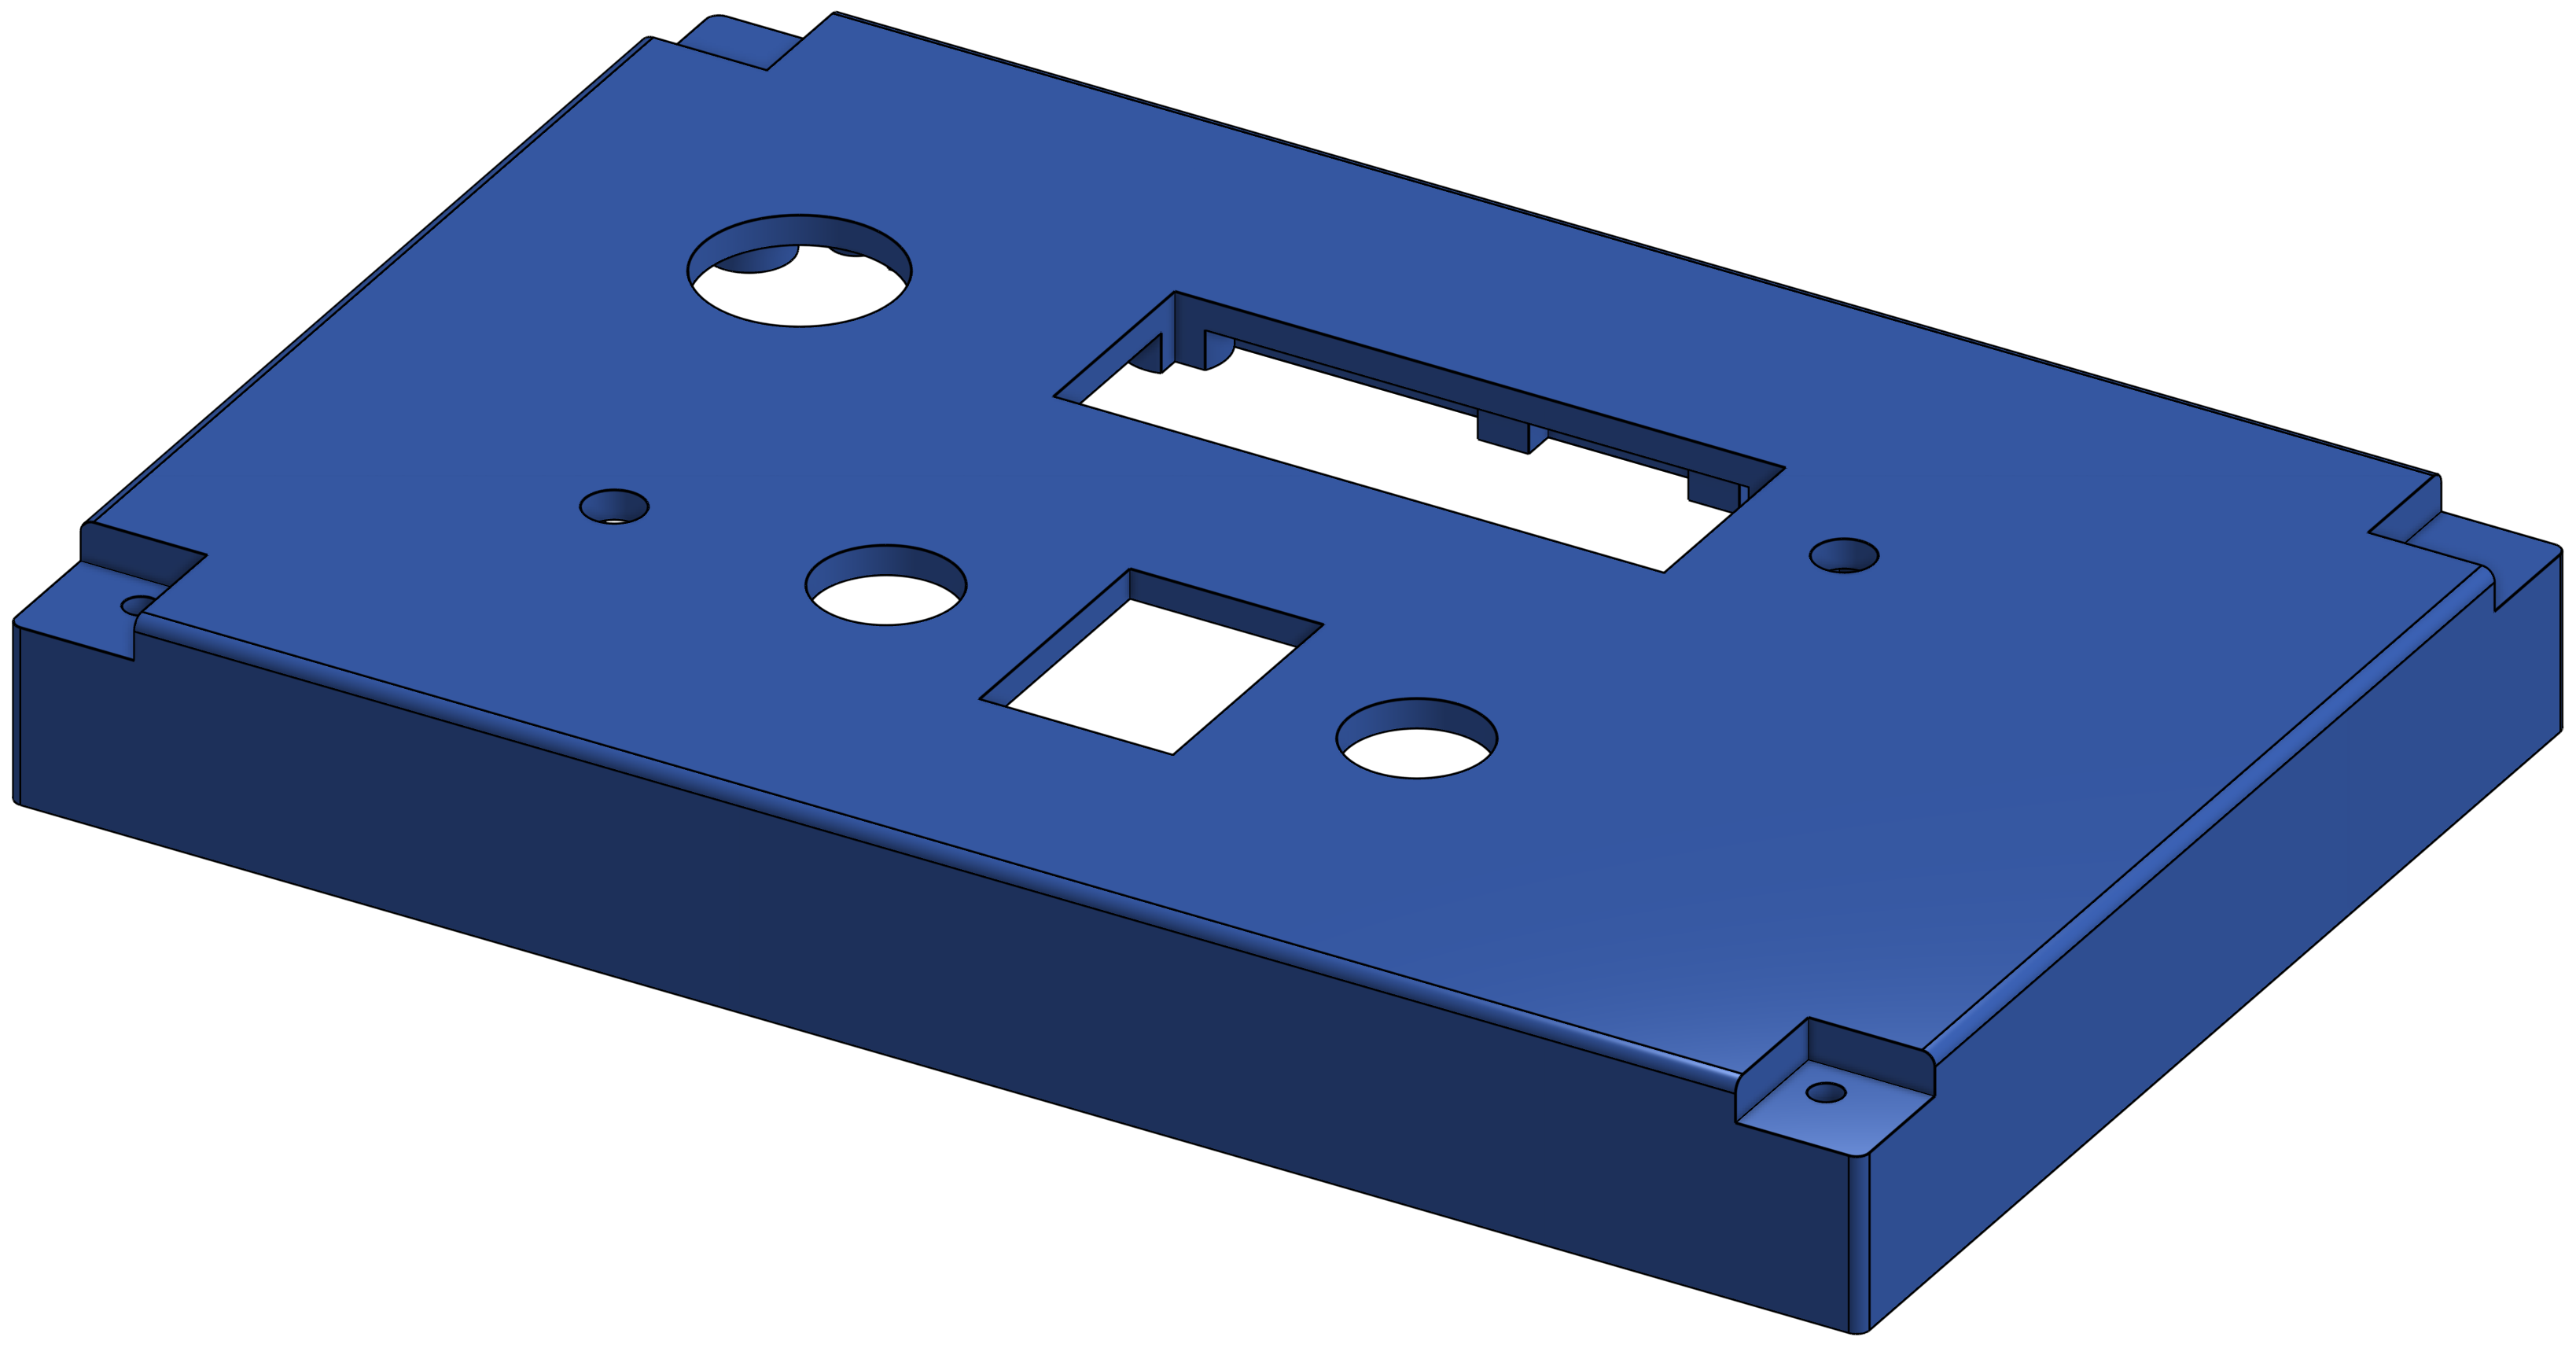
\includegraphics[width=0.5\textwidth]{04-caja/cajatapa.png}
    }% 
    \hspace{10pt}% 
    \subfloat[][]{% 
        \label{fig:cajatapaplanta}% 
        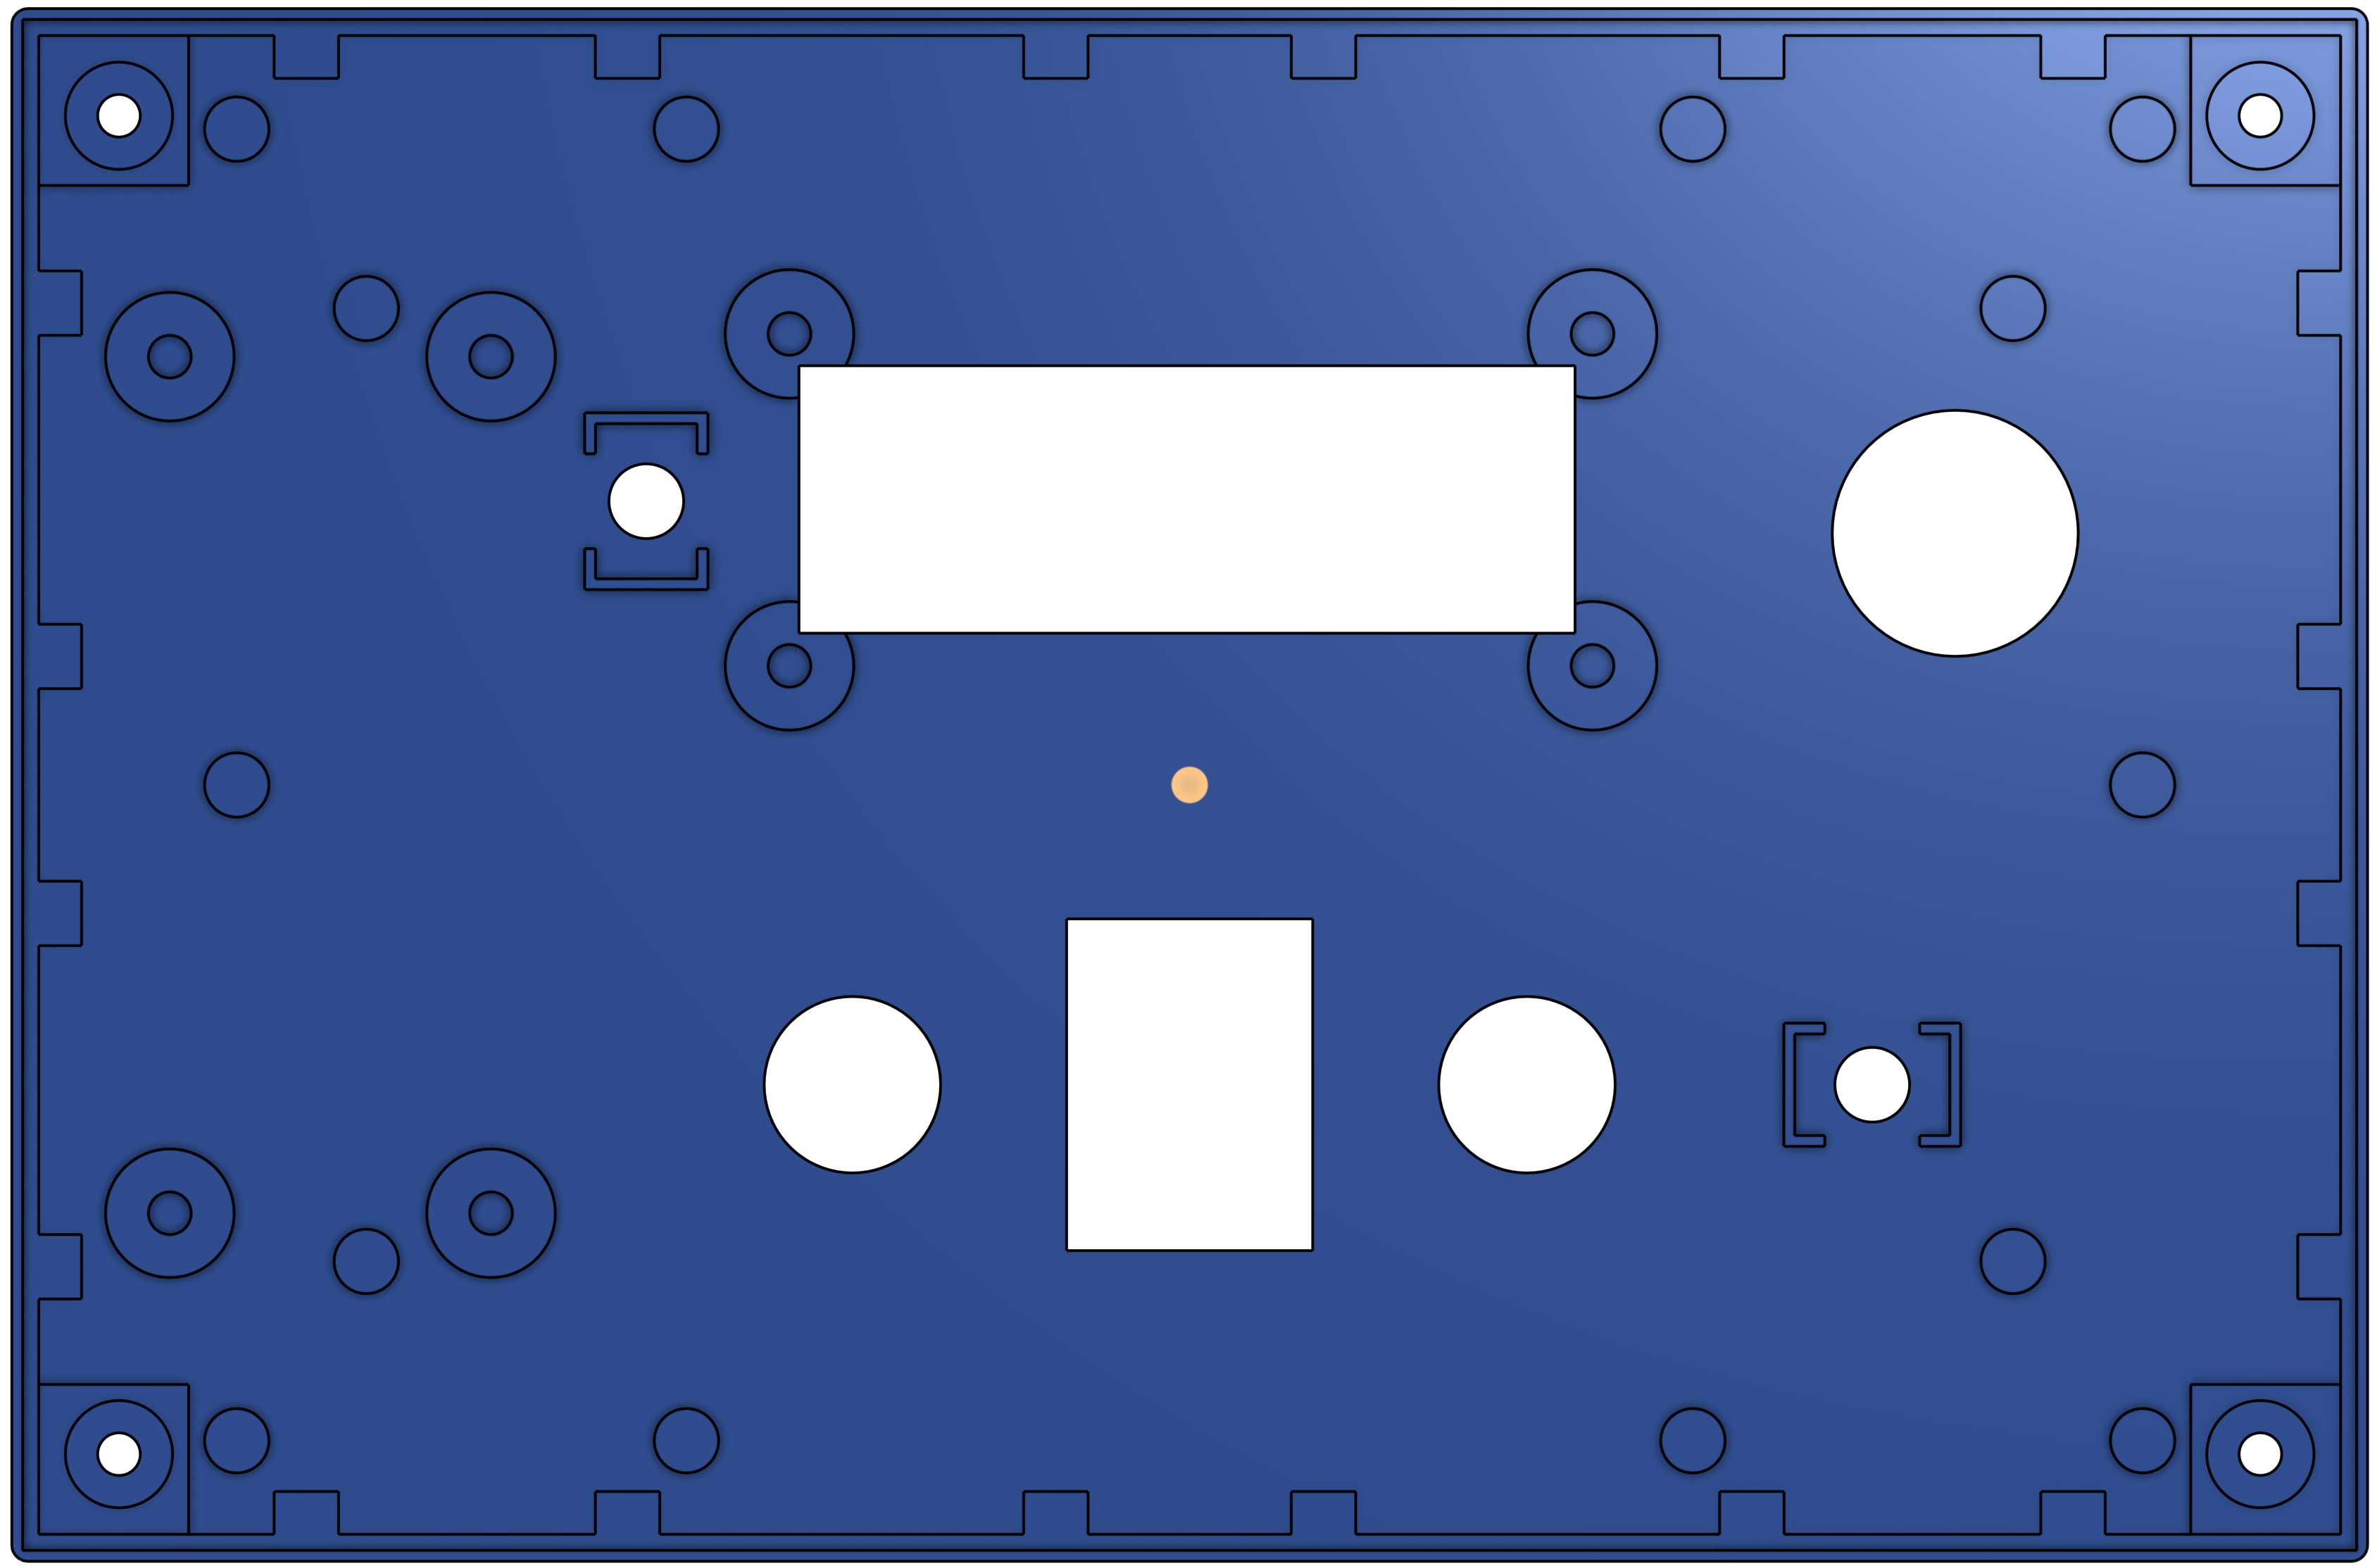
\includegraphics[width=0.5\textwidth]{04-caja/cajatapafondo.png}
    }
    \caption{a) Vista general de la tapa de la caja. b) Vista inferior de la tapa de la caja}
    \label{fig:cajatapa} 
\end{figure} 

Además, se muestra en la figura \ref{fig:cajatapaensamblaje} se muestra la distribución de los 
dispositivos. Ésta distribución permite cumplir con la planificación inicial que se observó en 
la figura \ref{fig:interfazhmi} y facilitar la conexión entre las placas electrónicas al colocar
la línea de interconexión de forma paralela.

\begin{figure}[h]%  
    \centering 
        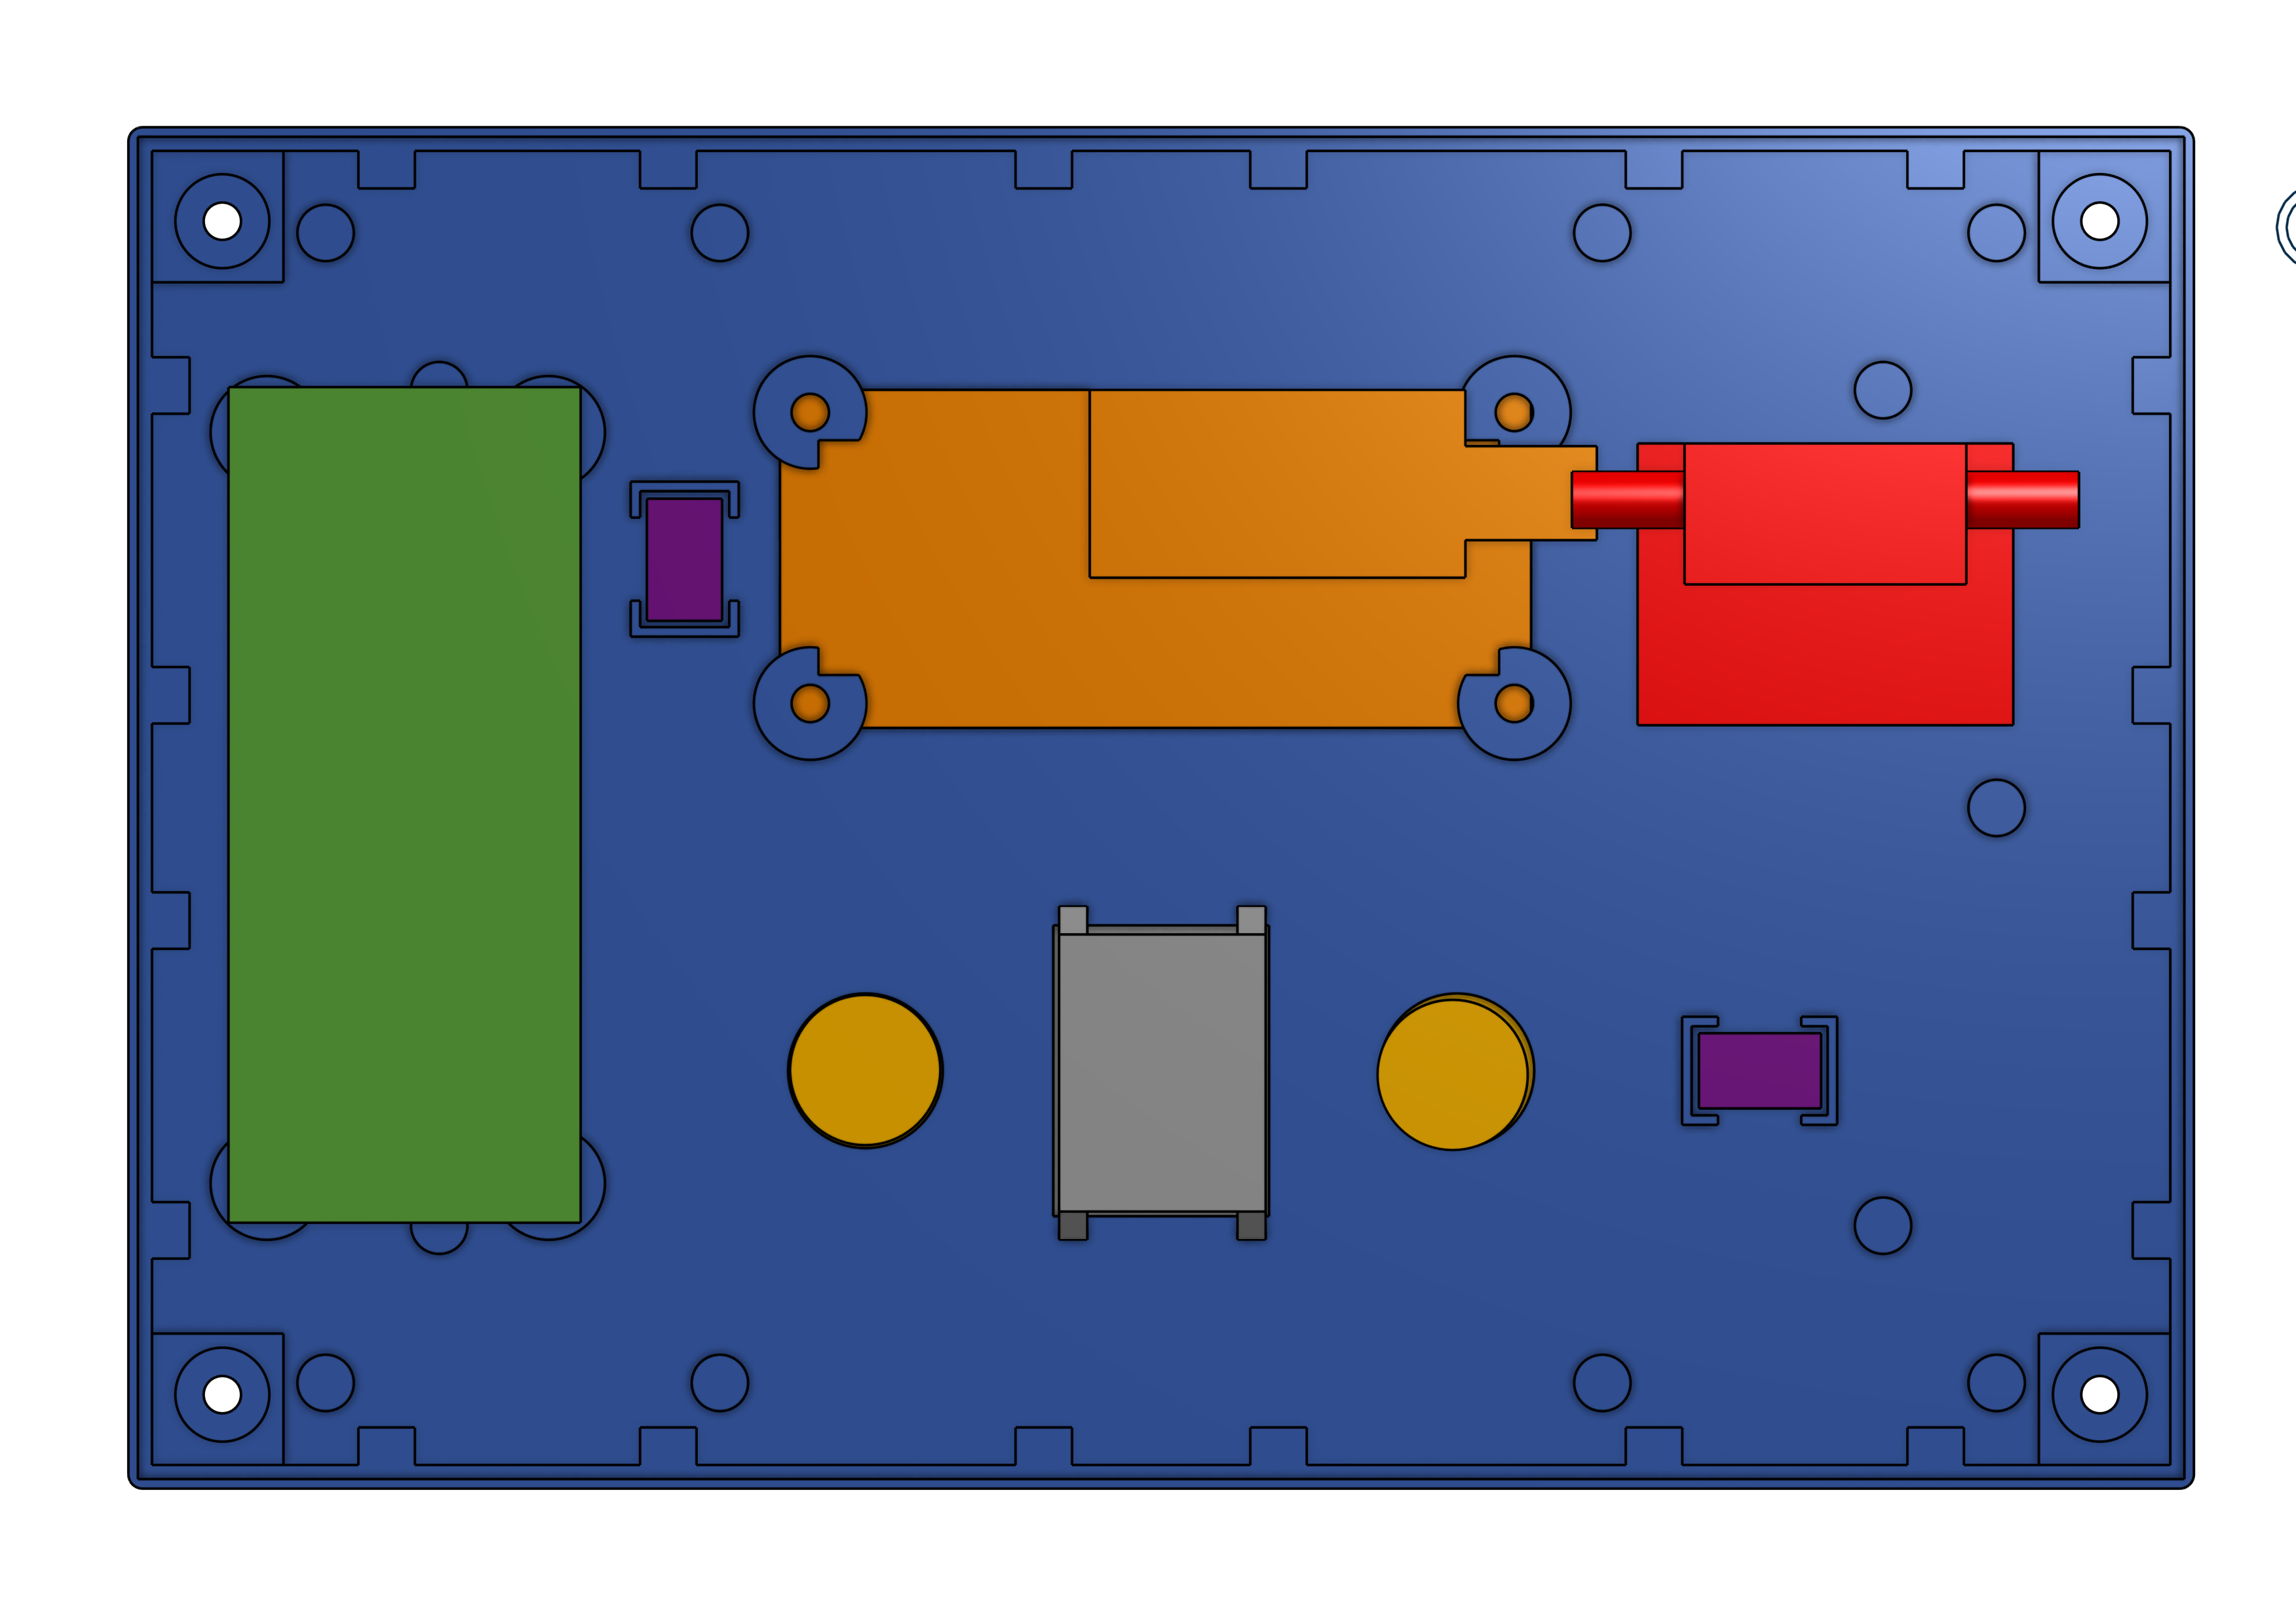
\includegraphics[width=0.5\textwidth]{04-caja/ensamblajetapainferior.png}
    \caption{Vista inferior de la tapa ensamblada. Descripción por colores: a) Verde: placa de 
    conexiones. b) Naranja: LCD c) Rojo: Seta de emergencia. d) Gris: Flechas de selección.
    e) Amarillo: Botones intro y escape. f) Morado: Selectores de modo}
    \label{fig:cajatapaensamblaje} 
\end{figure}
%
\chapter{Desarrollo en Arduino}\label{chp-05}

Una parte imprescindible del proyecto es la programación del propio Arduino, que es el que centraliza
todo el control del sistema. La parte relacionada con el control del motor y la programación del encoder 
está bien documentada en el trabajo \cite{tapia}, mientras que para la medición del calibre se ha partido
de la web \cite{caliper} al igual que en el diseño electrónico ya comentado en el capítulo \ref{chp-03}.

\section{Diagrama de flujo}

\begin{figure}[hbtp]
    \centering
    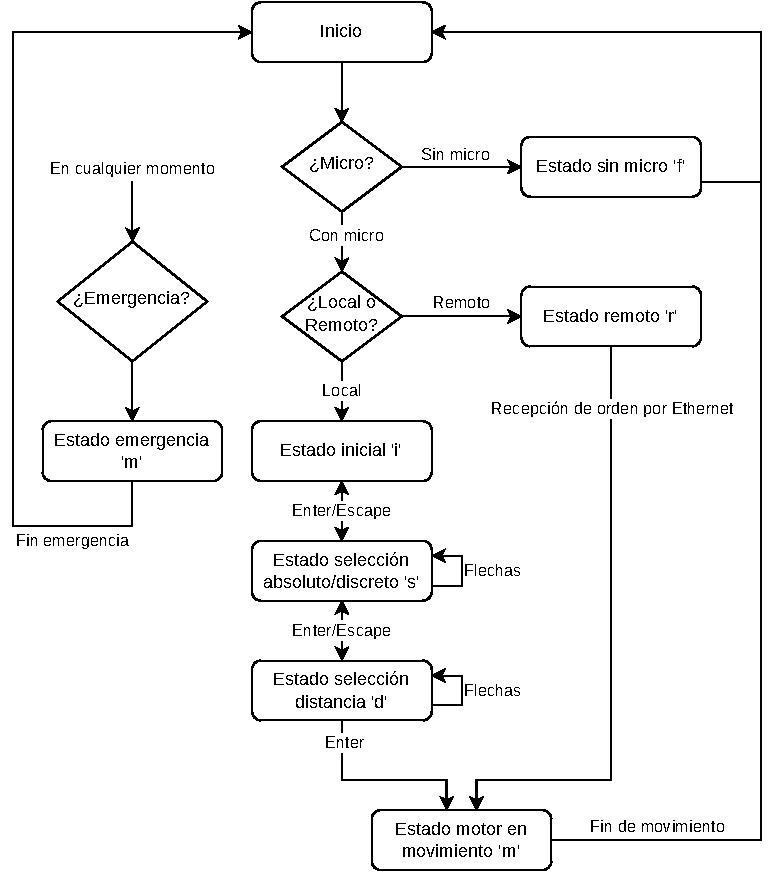
\includegraphics[height=0.5\textheight]{05-arduino/diagramaflujo.pdf}
    \caption{Diagrama de flujo del programa}
    \label{fig:diagramaflujo}
    \end{figure}

En el diagrama de la figura \ref{fig:diagramaflujo} se observa los distintos estados por los que pasa el 
programa. En primer lugar, se realiza una comprobación de los estados de microcontrolador y local para 
configurar los pines como corresponde. En caso de que no haya microcontrolador, se configurarán los pines
IN3, IN4 y ENB como entradas y el dispositivo esperará a que se salga de dicho modo, manteniéndose en estado 
"f". Si se configura como remoto, el Arduino entrará en estado "r" (remoto) y comprobará continuamente si se
recibe una orden por parte del controlador del ABB para realizar dicho movimiento.

El caso que tiene más estados intermedios es el modo local, ya que requiere varios menús dentro de la pantalla
para la interacción con el usuario. En este modo de funcionamiento se avanza en el menú con el botón enter y se
retrocede con el botón escape. Tras realizar las configuraciones del sistema, el sistema entrará en estado 
"i" (inicial), mostrado un mensaje de bienvenida en el LCD y esperando al botón enter para avanzar de menú. Una 
vez pulsado enter, se pasa al modo selección de avance absoluto o discreto, estado "s". En este estado, mediante
las flechas de selección se cambia entre avance discreto y avance absoluto. Una vez avanzado al siguiente menú, 
entramos en el modo selección de distancia de movimiento "d". En este modo, mediante las flechas se irá incrementando
o disminuyendo la posición final deseada. Por último, se tomará toda la información recibida por el usuario para 
pasar al estado de motor en movimiento "m".

Independientemente si se accede al estado "m" mediante modo local o remoto, la cinta se moverá hasta la posición 
deseada mediante el mismo algoritmo. Primero se aproxima la pieza a la posición final avanzando a velocidad constante
para posicionar finalmente la pieza mediante un PID. Una vez terminada la operación, vuelve al modo inicial para 
seguir esperando órdenes.

En cualquier caso, si en cualquier momento se pulsa la seta de emergencia, la cinta parará automáticamente y se entrará
en estado emergencia "e". En este modo no se podrá realizar ninguna acción hasta que se desarme la seta de emergencia.

\section{Programa final}

La pruebecita




\begin{lstlisting}[language=,caption={Declaración de variables, "main.h"}, breaklines=true, label=main_h]
// Definición de pines
#define faseA 2
#define faseB 3

#define BUTTON_ESC 22
#define BUTTON_ENTER 23
#define BUTTON_UP 24
#define BUTTON_DOWN 25

#define BUTTON_LOCAL 28
#define BUTTON_MICRO 29
#define BUTTON_EMERGENCIA 30

#define SENSOR_FOTO 31

#define CAL_CLK 32
#define CAL_DATA 33

#define ENB 5
#define IN3 40
#define IN4 41

// Declaración de objetos de LCD y relacionados con Ethernet
LiquidCrystal_I2C lcd(0x27,16,2);
byte MAC[] = { 0xDE, 0xAD, 0xBE, 0xEF, 0xFE, 0xED }; // Dirección MAC del dispositivo
EthernetServer servidor(4012); // Puerto donde se transmite la información

// Declaración de variables booleanas auxiliares
bool enter;
bool esc;
bool up;
bool down;
bool esc_ant = 0;
bool enter_ant = 0;
bool up_ant = 0;
bool down_ant = 0;

bool emergencia;
bool local;
bool micro;
bool fotoelectrico;

bool emergencia_ant;
bool local_ant;
bool micro_ant;

// Declaración e inicialización de variable de posición 'x' e 'y'
long posicion = 0;
long * pposicion = &posicion;
float posy = 0;

// Inicialización de variables de estado y desplazamiento
char estado = 'i';
bool discreto = 0;
long desplazamiento = 1000;
long objetivo = 0;

// Definición de parámetros de PID
float kp = 0.5;
float Ti = 2;
float Td = 0.1;
float T = 0.01;
    
\end{lstlisting}


blablabla


\begin{lstlisting}[language=,caption={Código principal Arduino, "main.ino"}, breaklines=true, label=main_cpp]
// Inclusión de librerías
#include <Ethernet.h>
#include <LiquidCrystal_I2C.h>
#include "main.h"

// Definición de funciones:

// Funciones de interrupción de encoder
void cambiofaseA(void);
void cambiofaseB(void);

// Funciones relacionadas al movimiento del motor
void pararMotor(void);
void moverMotor(void);
void movimientoMotor(long objetivo, long* posicion, LiquidCrystal_I2C lcd);

// Función de lectura del calibre digital
float medidaCalibre(void);

// Funciones de conexión por Ethernet
bool comprobarRobot(void);
bool enviarRobot(char dato);
void ethconex(void);

// Función setup de configuración del sistema
void setup() {
    // Inicializar el LCD
    lcd.init();
    
    // Encender la luz de fondo.
    lcd.backlight();
    
    // Definición de pines
    pinMode(faseA, INPUT_PULLUP);
    pinMode(faseB, INPUT_PULLUP);

    pinMode(BUTTON_DOWN, INPUT);
    digitalWrite(BUTTON_DOWN, HIGH);
    pinMode(BUTTON_UP, INPUT);
    digitalWrite(BUTTON_UP, HIGH);
    pinMode(BUTTON_ENTER, INPUT);
    digitalWrite(BUTTON_ENTER, HIGH);
    pinMode(BUTTON_ESC, INPUT);
    digitalWrite(BUTTON_ESC, HIGH);

    pinMode(BUTTON_EMERGENCIA, INPUT);
    pinMode(BUTTON_LOCAL, INPUT);
    pinMode(BUTTON_MICRO, INPUT);

    pinMode(SENSOR_FOTO, INPUT);

    // En función del estado de las señales MICRO, EMER y LR la configuración de IN3, IN4 y ENB pasa a INPUT u OUTPUT para evitar conflictos
    if(!digitalRead(BUTTON_MICRO)){
    pinMode(IN3, OUTPUT);
    pinMode(IN4, OUTPUT);
    pinMode(ENB, OUTPUT);
    if(!digitalRead(BUTTON_EMERGENCIA)){
        estado = 'i';
    } else{
        estado = 'e';
    }
    if(digitalRead(BUTTON_LOCAL)){
        estado = 'r';
    }
    } else{
    pinMode(IN3, INPUT);
    pinMode(IN4, INPUT);
    pinMode(ENB, INPUT);
    estado = 'f';
    }

    // Asociación de interrupción a los pines del encoder
    attachInterrupt(digitalPinToInterrupt(faseA), cambiofaseA, RISING);
    attachInterrupt(digitalPinToInterrupt(faseB), cambiofaseB, RISING);
    
    posy = medidaCalibre();
    posicion = 0;
    // Se inicia la comunicación Ethernet y la serie para depuración
    Ethernet.begin(MAC);
    Serial.begin(9600);
    Serial.print("Servidor en IP ");
    Serial.println(Ethernet.localIP());
}

// Bucle infinito
void loop() {

    // Se lee el estado de los botones
    up = digitalRead(BUTTON_UP);
    down = digitalRead(BUTTON_DOWN);
    enter = digitalRead(BUTTON_ENTER);
    esc = digitalRead(BUTTON_ESC);

    // Se lee el estado de la configuración
    emergencia = digitalRead(BUTTON_EMERGENCIA);
    local = digitalRead(BUTTON_LOCAL);
    micro = digitalRead(BUTTON_MICRO);

    // En el caso de cambio de las señales de modo o emergencia, pasar por setup() para reconfigurar los pines
    if(micro && (estado != 'f') && (estado != 'e')){
    setup();
    }

    if(local != local_ant){
    setup();
    }

    if(emergencia && (estado != 'e')){
    estado = 'e';
    lcd.clear();
    }

    // Máquina de estados
    switch(estado){
    // Estado inicial
    case 'i':
        lcd.setCursor(0, 0);
        lcd.print("MODO LOCAL      ");
        lcd.setCursor(0, 1);
        lcd.print("PULSE ENTER     ");
        digitalWrite(IN3, LOW);
        digitalWrite(IN4, LOW);
        analogWrite(ENB, 255);
        // Envío por Ethernet del estado al robot
        if(comprobarRobot()){
        enviarRobot(estado);
        }
        break;
        
    // Estado selección discreto/absoluto    
    case 's':
        lcd.setCursor(0, 0);
        lcd.print("SELECCIONE MOV. ");
        if(discreto){
        lcd.setCursor(0, 1);
        lcd.print("AVANCE DISCRETO ");
        } else{
        lcd.setCursor(0, 1);
        lcd.print("AVANCE ABSOLUTO ");
        }
        if(comprobarRobot()){
        enviarRobot(estado);
        }
        break;
        
    // Estado selección distancia de movimiento
    case 'd':
        if(comprobarRobot()){
        enviarRobot(estado);
        }
        break;
        
    // Estado movimiento del motor
    case 'm':
        if(comprobarRobot()){
        enviarRobot(estado);
        }
        movimientoMotor(objetivo, pposicion, lcd);
        if(comprobarRobot()){
        enviarRobot(estado);
        }
        posy = medidaCalibre();
        lcd.setCursor(0, 0);
        lcd.print("POSICION FINAL  ");
        lcd.setCursor(0, 1);
        lcd.print("                ");
        lcd.setCursor(0, 1);
        lcd.print("X=");
        lcd.print(posicion/10);
        lcd.print(" Y=");
        lcd.print(posy);
        delay(2000);
        estado = 'i';
        if(digitalRead(BUTTON_LOCAL)){
        estado ='r';
        }
        break;
        
    // Estado sin micro
    case 'f':
        lcd.setCursor(0, 0);
        lcd.print("SIN MICRO");
        break;
        
    // Estado emergencia
    case 'e':
        lcd.setCursor(0, 0);
        lcd.print("EMERGENCIA");
        break;
        
    // Estado remoto
    case 'r':
        lcd.setCursor(0, 0);
        lcd.print("MODO REMOTO     ");
        lcd.setCursor(0, 1);
        lcd.print("                ");
        digitalWrite(IN3, LOW);
        digitalWrite(IN4, LOW);
        analogWrite(ENB, 255);
        if(comprobarRobot()){
        enviarRobot(estado);
        }
        break;
    

    // Transiciones entre estados
    switch(estado){
    case 'i':
        if(!enter && enter_ant){
        estado = 's';
        }
        break;
        
    case 's':
        if(!enter && enter_ant){
        estado = 'd';
        
        posy = medidaCalibre();
        lcd.setCursor(0, 0);
        lcd.print("                ");
        lcd.setCursor(0, 1);
        lcd.print("                ");
        lcd.setCursor(0, 0);
        lcd.print("X=");
        lcd.print(posicion/10);
        lcd.print(" Y=");
        lcd.print(posy);

        lcd.setCursor(0, 1);
        if(desplazamiento > 0){
            lcd.print("+");
        }
        lcd.print(desplazamiento/10);
        lcd.print(" mm");                
        }
        if(!esc && esc_ant){
        estado = 'i';
        }
        if((!up && up_ant) || (!down && down_ant)){
        discreto = !discreto;
        }
        break;

    case 'd':
        if(!enter && enter_ant){
        estado = 'm';
        if(discreto){
            objetivo = posicion + desplazamiento;
        } else{
            objetivo = desplazamiento;
        }
        }
        if(!esc && esc_ant){
        estado = 's';
        }
        if(!up && up_ant){
        desplazamiento = desplazamiento + 1000;
        lcd.setCursor(0, 1);
        lcd.print("                ");
        lcd.setCursor(0, 1);
        if(desplazamiento > 0){
            lcd.print("+");
        }
        lcd.print(desplazamiento/10);
        lcd.print(" mm");        
        }
        if(!down && down_ant){
        desplazamiento = desplazamiento - 1000;
        lcd.setCursor(0, 1);
        lcd.print("                ");
        lcd.setCursor(0, 1);
        if(desplazamiento > 0){
            lcd.print("+");
        }
        lcd.print(desplazamiento/10);
        lcd.print(" mm");        
        }
        break;

    case 'f':
        if(!micro){
        setup();
        }
        break;

    case 'e':
        if(!emergencia){
        setup();
        }
        break;
    }

    // Guardado de estados
    esc_ant = esc;
    enter_ant = enter;
    up_ant = up;
    down_ant = down;
    
    emergencia_ant = emergencia;
    local_ant = local;
    micro_ant = micro;
    
    delay(10);
}

// Funciones definidas en la cabecera

// Si hay cambio en la fase A, se comprueba la fase B para definir el sentido de giro
void cambiofaseA(void){
    bool fB = digitalRead(faseB);
    if(fB){
    posicion++;
    } else{
    posicion--;
    }
}

// Si hay cambio en la fase A, se comprueba la fase B para definir el sentido de giro
void cambiofaseB(void){
    bool fA = digitalRead(faseA);
    if(fA){
    posicion--;
    } else{
    posicion++;
    }
}

// Parado de motor
void pararMotor(void){
    digitalWrite(IN3, LOW);
    digitalWrite(IN4, LOW);
    analogWrite(ENB, 255);
}

// Avance de motor a la velocidad especificada
void moverMotor(int u){
    if(u >= 0){ // Avance positivo
        digitalWrite(IN3, LOW);
        digitalWrite(IN4, HIGH);
    } else{ // Avance negativo
        digitalWrite(IN3, HIGH);
        digitalWrite(IN4, LOW);
        u = -u;
    }

    if(u > 200){
        u = 200; // La salida máxima es de 255 pero se limita a 200
    }

    analogWrite(ENB, u);
}

// Función que coloca el sistema en la posición deseada
void movimientoMotor(long objetivo, long* posicion, LiquidCrystal_I2C lcd){
    lcd.setCursor(0, 0);
    lcd.print("MOVIENDO...     ");
    lcd.setCursor(0, 1);
    lcd.print("                ");
    lcd.setCursor(0, 1);
    lcd.print((*posicion)/10);
    lcd.print("/");
    lcd.print(objetivo/10);

    long u = 0;
    long ek = 0;
    long ek1 = 0;
    long ik = 0;
    long D = 0;
    int aux = 0;
    bool emer = 0;
    
    // Bucle PID. Se mantiene buscando la posición mientras no entre dentro de un margen y la acción de control no se encuentre por debajo del umbral de funcionamiento
    while(((*posicion < objetivo - 5) || (*posicion > objetivo + 5) || (u > 55)) && !emer){
    
    emer = digitalRead(BUTTON_EMERGENCIA);

    // Se actualiza la posición actual en el LCD cada 120 ms
    aux++;
    if(aux > 3){
        lcd.setCursor(0, 1);
        lcd.print("                ");
        lcd.setCursor(0, 1);
        lcd.print((*posicion)/10);
        lcd.print("/");
        lcd.print(objetivo/10);        
        aux = 0;
    }

    //Actualización de error integral
    ek1 = ek;
    ek = objetivo - *posicion;
    ik = ik + ek;
    D = ek - ek1;
    //Cálculo de la señal de control
    u = kp * (ek + (T/Ti) * ik + (Td/T) * D);
    
    // En caso de saturación, reiniciar el error integral
    if((abs(u) > 255) && (abs(ek) > 200)){
        ik = 0;
    }

    // Limitar la acción de control al máximo que permite Arduino
    if(u > 255){
        u = 255;
    }
    if(u < -255){
        u = -255;
    }
    
    if(!emer){
        moverMotor(u);
        delay(1000 * T);
    }
    }
    
    // Parar el motor cuando se alcance la posición deseada
    pararMotor();
    
    if(emer){
    lcd.clear();
    lcd.print("EMERGENCIA");
    delay(1000*T);
    }
}

// Medida del calibre
float medidaCalibre(void){
    bool data;
    float medida;
    int value = 0;
    int signo = 0;

    unsigned long tempmicros;
    unsigned long tempmicros2;

    // Reintentar la medición hasta que se pueda realizar
    for(int j=0; j<10 && (value == 0); j++){

    tempmicros = micros();
    while (digitalRead(CAL_CLK)==LOW) {
        delayMicroseconds(1);      
    }

    tempmicros2 = micros();
    if ((tempmicros2-tempmicros)>10000) {
        // Se leen los 24 bits que proporciona el calibre
        for (int i=0; i<24; i++) {
        while (digitalRead(CAL_CLK)==HIGH) {
            delayMicroseconds(1);
        }

        data = !digitalRead(CAL_DATA);
    
            // Se leen los datos cada bajada del flanco de reloj
        if(i<16){
            value |= data << i;
        }else{
            signo |= (data << (i-16));
        }

        while (digitalRead(CAL_CLK)==LOW) {
            delayMicroseconds(1);
        }
        }
        
        // El bit 0x80 corresponde a las unidades, pulgadas o milímetros
        // En caso de que sean pulgadas, se realiza la conversión a milímetros
        if(signo & 0x80){
        medida = 25.4*float(value)/(2*1000);
        } else{
        medida = float(value)/100;
        } 

        // El bit 0x10 corresponde al signo
        if(signo & 0x10){
        medida = -medida;
        }
    }
    }
    return medida;
}

// Comprobación de que existe una conexión con el robot
// Devuelve 1 si se produce la conexión y 0 en caso contrario
bool comprobarRobot(void){
    EthernetClient cliente = servidor.available();
    if (cliente) {
    return 1;
    } else{
    cliente.stop();
    return 0;
    }
}

// Función para enviar estado del sistema, sensor fotoélectrico y recibir la orden de movimiento del propio robot
// El robot envía la orden, ya sea de recibir el estado del sistema o el movimiento deseado
// Una vez recibido, el Arduino envía los datos necesarios y mueve la cinta si se encuentra en estado remoto
bool enviarRobot(char dato){
    EthernetClient cliente = servidor.available();
    String recepcion;
    if (cliente) {
    while (cliente.connected()) {
        if (cliente.available()) {
        recepcion = cliente.readString();
        Serial.println(recepcion);
        if(recepcion == "STATUS"){
            String envio = (String) dato + ";X=" + String(posicion, 2) + ";Y=" + String(posy, 2);
            String fotoele = ";F=" + String(digitalRead(SENSOR_FOTO));
            envio = envio + fotoele;
            cliente.println(envio);
            Serial.println(recepcion);
        }
        if(recepcion.indexOf('M') > -1){
            if(estado == 'r'){
            int igual_pos = recepcion.indexOf("=");
            int fin_pos = recepcion.indexOf(";",igual_pos);
            String movimiento = recepcion.substring(igual_pos+1, fin_pos);
            objetivo = movimiento.toInt();
            estado = 'm';
            }
        }
        if(recepcion.indexOf('R') > -1){
            if(estado == 'r'){
            int igual_pos = recepcion.indexOf("=");
            int fin_pos = recepcion.indexOf(";",igual_pos);
            String movimiento = recepcion.substring(igual_pos+1, fin_pos);
            objetivo = movimiento.toInt() + posicion;
            estado = 'm';
            }
        }
        }
    }
    cliente.stop();
    }
    return 0;
}    
\end{lstlisting}
%
\chapter{Desarrollo en Robotstudio}\label{chp-06}

La idea principal del proyecto es orientar el sistema para la realización de prácticas de 
laboratorio, por lo que el trabajo a realizar por los alumnos está en la programación en 
Robotstudio. Por esta razón, este capítulo va orientado a dar las pautas necesarias para el 
funcionamiento del sistema y su integración en el ecosistema de ABB.

\section{Funcionamiento sin microcontrolador}

El caso más simple de funcionamiento es cuando no hay microcontrolador. En este caso se
utilizarán las entradas y salidas digitales del controlador para realizar los movimientos.
La conexión entre las salidas digitales de la caja y el controlador se realiza mediante 
un módulo de interfaz como el mostrado en la figura \ref{fig:interfazfisicadigital}.

\begin{figure}[hbtp]
    \centering
    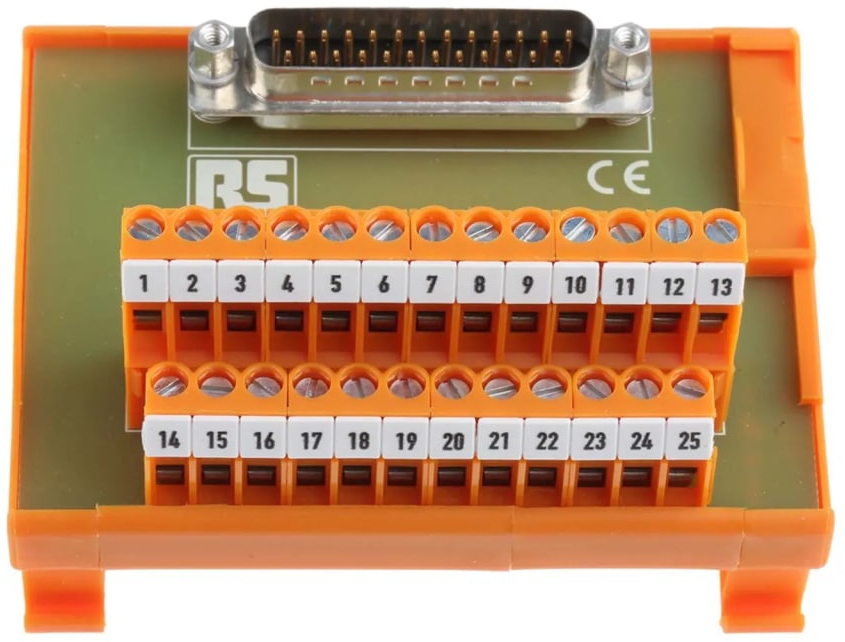
\includegraphics[width=\textwidth/2]{06-robotstudio/interfazdigital.jpg}
    \caption{Amplificación señales calibre digital a 5V}
    \label{fig:interfazfisicadigital}
    \end{figure}

Dicho módulo se conecta a la placa DSQC 652 que se encuentra montada en el controlador del robot.
Este dispositivo está diseñado para manejar señales digitales entre el sistema del robot y sistemas
como el de este proyecto. Los pines expuestos en el módulo de interfaz son los siguientes:
\begin{itemize}
    \item Entradas (DI, Digital Inputs). Pines del 1 al 8 que corresponden a los DI01 a DI08.
    \item Salidas (DO, Digital Outputs). Pines del 14 al 24 que corresponden a los DO01 a DO08.
    \item GND. Pin 24.
    \item VCC 24V. Pin 25.
\end{itemize}

En el los pines de salida se conectarán las señales de Avance y Retroceso, mientras que en los
de entrada estarán la señal del sensor fotoeléctrico, la emergencia, el estado de la señal local y
la señal micro.

Las funciones referentes a las señales digitales se pueden consultar en el manual de RAPID \cite{rapid}.
Las más relevantes para el uso básico son:
\begin{itemize}
    \item SetDO, cambio de valor en salida digital. Uso: SetDo señalDO, valor;
    \item Lectura de entrada digital. Se puede realizar simpelmente utilizando el nombre de la señal. 
    Usos: estado-actual := señalDI; IF señalDI = valor DO ...
    \item WaitDI, espera en el programa hasta que una señal de entrada tome cierto valor.
    Uso: WaitDI señalDI, valor;
\end{itemize}

Un ejemplo de programa es el que se puede ver en \ref{no_micro}. Este programa consiste en hacer avanzar
la cinta hasta que se enciende el sensor fotoeléctrico, que el robot recoja la pieza y repita la operación
haciéndolo retroceder. Para ello, se debe definir el \textit{workobject} de la cinta transportadora para mover
el brazo robótico sobre sus ejes. Posteriormenete se debe definir la posición de recogida del brazo donde 
se activa el sensor fotoeléctrico. Las demás posiciones se generarán mediante offsets de la posición de recogida.
El trabajo con el brazo robótico queda a cargo de futuros alumnos, aquí se muestra exclusivamente el trato 
con las señales digitales. Para simplificar los nombres de las señales se utilizan nombres descriptivos, no
el que realmente aparece en RobotStudio.

\begin{lstlisting}[language=,caption={Ejemplo de programa sin microcontrolador}, breaklines=true, label=no_micro]
MODULE Module1
    !Aquí deben estar definidas las posiciones y variables auxiliares
    !
    PROC main()
        !Se procede a avanzar 
        SetDO señalAvance, 1;
        SetDO señalRetroceso, 0;

        !Se espera a que se active el sensor fotoeléctrico
        WaitDI señalFoto, 1;
        !Se para la cinta
        SetDO señalAvance, 0;
        SetDO señalRetroceso, 0;
        
        !Movimiento del brazo robótico para recoger la pieza y colocarla en una posición avanzada donde haya que retroceder
        ...

        !Misma operación a la inversa
        SetDO señalAvance, 0;
        SetDO señalRetroceso, 1;

        !Se espera a que se active el sensor fotoeléctrico
        WaitDI señalFoto, 1;
        !Se para la cinta
        SetDO señalAvance, 0;
        SetDO señalRetroceso, 0;

        !Movimiento del brazo robótico para recoger la pieza y colocarla en la posición original
        ...
    ENDPROC
END MODULE
\end{lstlisting}

\section{Funcionamiento con microcontrolador}
%
\chapter{Resultados}\label{chp-07}

FOTOS:

CAJA ENCENDIDA

CAJA TRASERA

CAJA INTERIOR

CAJA EXTERIOR

PLACA FONDO

PLACA TAPA
%
\chapter{Conclusiones}\label{chp-08}



%:Empezamos con los apéndices, que irían en uno o más ficheros. Es necesario incluir estos ficheros entre el entorno \begin{appendices}....\end{appendices} debido a que se ha deseado utilizar un formato diferente para el título de los apéndices, incluyendo la palabra apéndice, para la numeración de los apéndices, alfabético, y para las cabeceras de las páginas.
%
%\begin{appendices}
%
%% !TEX root =../LibroTipoETSI.tex



%APENDICE A
\chapter{Sobre  \LaTeX}\LABAPEN{ApA}
{Este es un ejemplo de apéndices, el texto es únicamente relleno, para que el lector pueda observar cómo se utiliza}
%%%%%%%%%%%%%%%%%
\section{Ventajas de \LaTeX}

El gusto por el \LaTeX\ depende de la forma de trabajar de cada uno. La principal virtud es la facilidad de formatear cualquier texto y la robustez. Incluir títulos, referencias es inmediato.
%\Blindtext
%\lipsum
Las ecuaciones quedan estupendamente, como puede verse en \EQ{Ap1}
\begin{equation}\LABEQ{Ap1}
x_{1}=x_{2}.
\end{equation}


\section{Inconvenientes}
%\Blindtext
El principal inconveniente de \LaTeX\ radica en la necesidad de aprender un conjunto de comandos para generar los elementos que queremos. Cuando se está acostumbrado a un entorno ``como lo escribo se obtiene'', a veces resulta difícil dar el salto a ``ver'' que es lo que se va a obtener con un determinado comando. 

Por otro lado, en general será muy complicado cambiar el formato para desviarnos de la idea original de sus creadores. No es imposible, pero sí muy difícil. Por ejemplo, con la sentencia siguiente:
 
\begin{lstlisting}[language=,caption={Escritura de una ecuación}, breaklines=true, label=prgA1-01]
\begin{equation}\LABEQ{Ap2}
x_{1}=x_{2}
\end{equation}
\end{lstlisting}
obtenemos:
\begin{equation}\LABEQ{Ap2}
x_{1}=x_{2}
\end{equation}
Esto será siempre así. Aunque, tal vez, esto podría ser una ventaja y no un incoonveniente.

Para una discusión similar sobre el Word\tsp{\textregistered}, ver \APEN{ApB}.
%\Blindtext


%%%%%%%%%%%%%%%%%%%%%%%%%%%%%%%%%%%%%%%
%APENDICE B
\chapter{Sobre Microsoft Word\tsp{\textregistered}}\LABAPEN{ApB}

\section{Ventajas del Word\tsp{\textregistered}}
La ventaja mayor del Word\tsp{\textregistered} es que permite configurar el formato muy fácilmente. Para las ecuaciones,
\begin{equation}
x_{1}=x_{2},
\end{equation}
tradicionalmente ha proporcionado pésima presentación. Sin embargo, el software adicional Mathtype\tsp{\textregistered} solventó este problema, incluyendo una apariencia muy profesional y cuidada. Incluso permitía utilizar un estilo similar al \LaTeX\xspace. Además, aunque el Word\tsp{\textregistered} incluye sus propios atajos para escribir ecuaciones,  Mathtype\tsp{\textregistered} admite también escritura \LaTeX\xspace. En las últimas versiones de Word\tsp{\textregistered}, sin embargo, el formato de ecuaciones está muy cuidado, con un aspecto similar al de \LaTeX.


\section{Inconvenientes de Word\tsp{\textregistered}}
Trabajar con títulos, referencias cruzadas e índices es un engorro, por no decir nada sobre la creación de una tabla de contenidos. Resulta muy frecuente que alguna referencia quede pérdida o huérfana y aparezca un mensaje en negrita indicando que  no se encuentra. 

Los estilos permiten trabajar bien definiendo la apariencia, pero también puede desembocar en un descontrolado incremento de los mismos. Además, es muy probable que Word\tsp{\textregistered} se quede colgado, sobre todo al trabajar con copiar y pegar de otros textos y cuando se utilizan ficheros de gran extensión, como es el caso de un libro.

%\end{equation}
 
%
%\end{appendices}

%%%%%%%%%%%%%%%%%%%%%%%%%%%%%%%%%%%%%%
%%%%%%%%%%%%%%%%%%%%%%%%%%%%%%%%%%%%%%
%:Empieza todo lo que no constituye el cuerpo en si del libro. Todo lo que va detrás
\backmatter

%:Indice de figuras, coméntese las siguientes líneas si no se desea
\cleardoublepage
\phantomsection

%:Para añadir una línea en blanco en el TOC y separar esta lista
\addtocontents{toc}{\protect\mbox{}\protect\hspace*{0pt}\par}
\addcontentsline{toc}{listasb}{\listfigurename}
\pagestyle{especial}
\listoffigures

%:Indice de tablas, coméntese las siguientes líneas si no se desea
\cleardoublepage
\phantomsection
\addcontentsline{toc}{listasb}{\listtablename}
\pagestyle{especial}
\listoftables

%:Indice de Programas
\cleardoublepage
\phantomsection
\addcontentsline{toc}{listasb}{\lstlistlistingname}
\pagestyle{especial}
\lstlistoflistings

%:Bibliografía con biblatex
\cleardoublepage
\phantomsection
\addcontentsline{toc}{listasb}{\bibname}
\pagestyle{especial}

%\bibliographystyle{IEEEtran}
\bibliographystyle{amsplain} %flexbib amsplain alpha

%:Fichero con la bibliografía, BIBTEX
\bibliography{bibliografiaLibroETSI}

% Este fichero .bib se puede generar usando algún gestor de bibliografías. Se recomiendan dos:
% - Zotero
% - Mendeley (con licencia de la US)

%:Índice alfabético de palabras
%\cleardoublepage
%\phantomsection
%\addcontentsline{toc}{listasb}{\indexname}
%\chaptermark{\indexname}
%\printindex


%:Acrónimos
%\cleardoublepage
%\phantomsection
%\addcontentsline{toc}{listasb}{\glossaryname}
%\chaptermark{\glossaryname}
%\printglossaries


\end{document}